\documentclass[12pt]{report}
\usepackage{graphicx}
\usepackage{hyperref}
\usepackage{geometry}
\usepackage{amsmath}
\usepackage{booktabs}
\usepackage{longtable}
\usepackage{array}
\usepackage{float}
\usepackage{caption}
\usepackage{tikz}
\usetikzlibrary{positioning}
\usepackage{listings}
\usepackage{setspace}
\geometry{margin=1in}
\onehalfspacing

\title{International Migration Network Analysis\\A Network Science and Machine Learning Project}
\author{Jaswinder Singh (ID: 12340970)\\Aditya Yadav (ID: 12340100)\\Dipanjan Mondal (ID: 12340670)}
\date{April 2026}

\begin{document}
\maketitle

\begin{abstract}
This report delivers a structured, end-to-end analysis of global migration using network science and machine learning. Countries are modeled as nodes and migration flows as directed weighted edges across eight snapshots (1990--2024). The study combines dynamic network construction, centrality metrics, community evolution, temporal drift measures, and regression modeling. We introduce a custom Migration Influence Score (MIS) that blends PageRank with total flow volume to surface practical hubs. Outputs include tables, figures, and dashboard-ready artifacts to support interpretation and presentation.
\end{abstract}

\tableofcontents
\listoffigures
\listoftables
\newpage

\chapter*{Executive Summary}
\addcontentsline{toc}{chapter}{Executive Summary}
\begin{itemize}
    \item Built 8 dynamic migration networks (1990--2024) from UN DESA data.
    \item Identified global hubs using centrality and a custom MIS metric.
    \item Measured community stability using NMI, ARI, and Jaccard drift.
    \item Achieved strong predictive performance with regression models ($R^2 \approx 0.95$).
    \item Delivered dashboards and reproducible artifacts for reporting.
\end{itemize}
\clearpage

\chapter{Introduction}
International migration reshapes demographics, economies, and policy. Network science provides a systems view of migration by modeling countries as nodes and flows as directed weighted edges. This report focuses on structural hubs, community evolution, and temporal stability, and extends the analysis with machine learning and a custom influence metric.

\chapter{Problem Statement and Objectives}
\section{Problem Statement}
How can migration from 1990 to 2024 be modeled as a dynamic network to reveal hubs, community structure, and temporal drift, while linking flows to explanatory features?

\section{Objectives}
\begin{itemize}
    \item Build a dynamic directed migration network for multiple snapshots.
    \item Compute centrality metrics to identify origin and destination hubs.
    \item Detect communities and quantify stability over time.
    \item Introduce a custom influence metric for practical ranking.
    \item Train regression models to evaluate predictive relationships.
    \item Produce reproducible outputs and dashboards.
\end{itemize}

\chapter{Dataset and Preprocessing}
\section{Data Sources}
\textbf{Primary:} UN DESA International Migrant Stock 2024.\\
\textbf{Auxiliary (when available):} GDP, population, unemployment, conflict indicators.

\section{Preprocessing Workflow}
\begin{itemize}
    \item Removed aggregate/non-country rows and standardized country identifiers.
    \item Converted matrix-form data to long-format origin--destination--year rows.
    \item Validated numeric ranges and handled missing values.
\end{itemize}

\section{Snapshot Summary}
\begin{table}[H]
\centering
\caption{Snapshot Summary (Nodes, Edges, Total Migrants)}
\label{tab:snapshot-summary}
\begin{tabular}{lrrr}
\toprule
Year & Nodes & Edges & Total Migrants \\
\midrule
1990 & 234 & 8235 & 153,916,063 \\
1995 & 234 & 8468 & 163,176,002 \\
2000 & 234 & 8593 & 174,566,152 \\
2005 & 234 & 8727 & 192,788,721 \\
2010 & 234 & 9013 & 221,020,392 \\
2015 & 234 & 9264 & 250,042,020 \\
2020 & 234 & 9269 & 275,284,032 \\
2024 & 234 & 9273 & 304,021,813 \\
\bottomrule
\end{tabular}
\end{table}

\chapter{Exploratory Analysis}
Migration flows are heavy-tailed: a small number of countries dominate inflow and outflow. The most intense corridors are highly concentrated, indicating structural hubs and persistent routes.

\section{Top Destinations (2024)}
\begin{itemize}
    \item United States of America* (52,375,047)
    \item Germany (16,750,084)
    \item Saudi Arabia (13,683,841)
    \item United Kingdom* (11,845,479)
    \item France* (9,186,757)
\end{itemize}

\section{Top Origins (2024)}
\begin{itemize}
    \item India (18,533,845)
    \item China (11,701,619)
    \item Mexico (11,596,529)
    \item Ukraine* (9,769,216)
    \item Russian Federation (9,134,094)
\end{itemize}

\section{Top Corridors (2024)}
\begin{itemize}
    \item Mexico $\rightarrow$ United States of America* (11,279,561)
    \item Afghanistan $\rightarrow$ Iran (3,752,317)
    \item Syrian Arab Republic $\rightarrow$ T\"urkiye (3,563,983)
    \item Russian Federation $\rightarrow$ Ukraine* (3,375,095)
    \item India $\rightarrow$ United Arab Emirates (3,248,545)
\end{itemize}

\chapter{Methodology}
\section{Network Model}
Migration is modeled as a directed weighted graph $G=(V,E)$, where nodes are countries and edge weights represent migration stock.

\section{Pipeline Flow Diagram}
\begin{figure}[H]
\centering
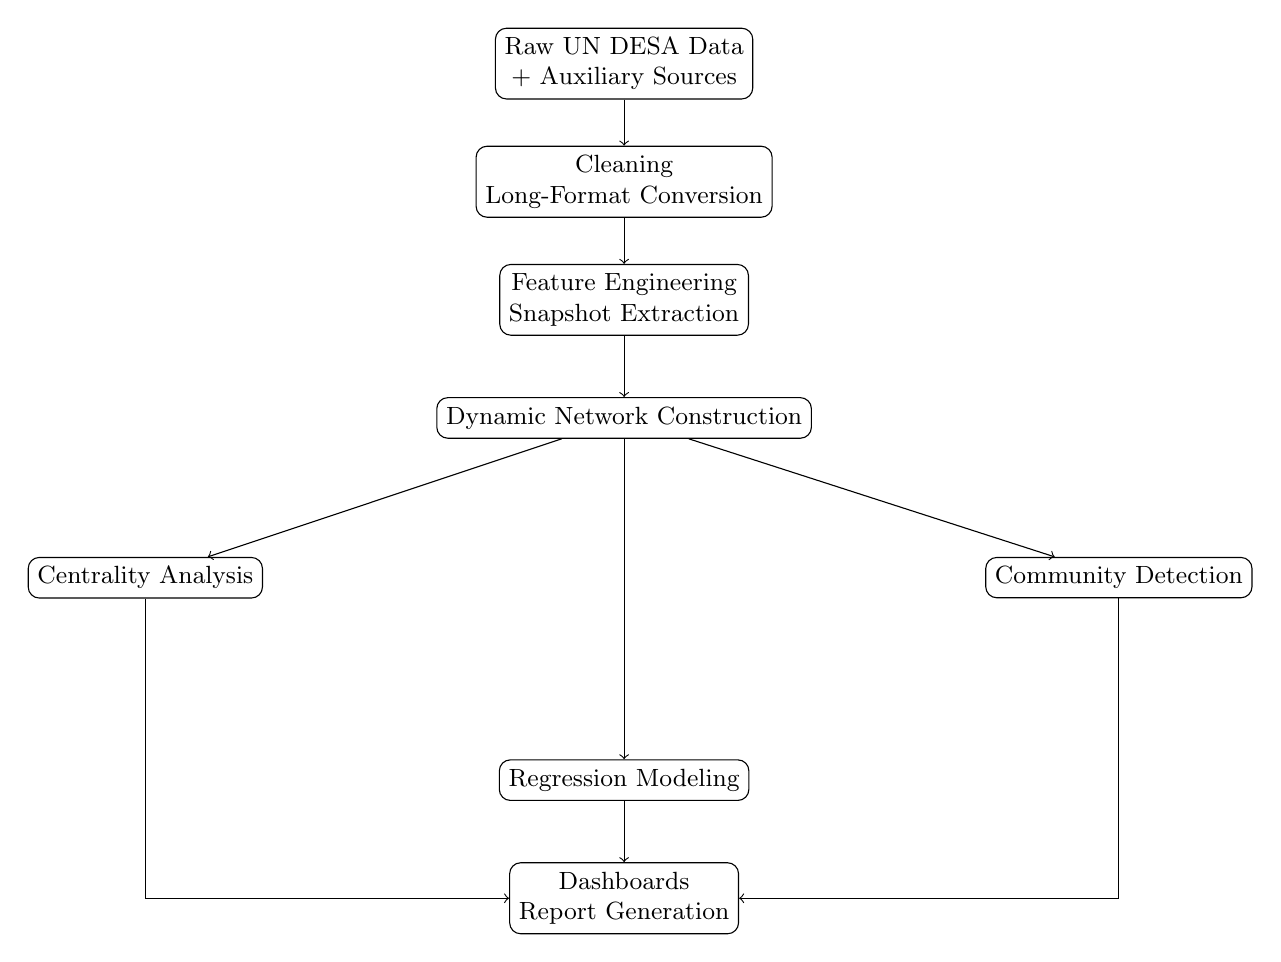
\begin{tikzpicture}[node distance=1.5cm, every node/.style={draw, rounded corners, align=center, font=\small}]
\node (data) {Raw UN DESA Data\\+ Auxiliary Sources};
\node (clean) [below of=data] {Cleaning \\ Long-Format Conversion};
\node (features) [below of=clean] {Feature Engineering \\ Snapshot Extraction};
\node (network) [below of=features] {Dynamic Network Construction};
\node (centrality) [below left=1.5cm and 2.2cm of network] {Centrality Analysis};
\node (community) [below right=1.5cm and 2.2cm of network] {Community Detection};
\node (regression) [below of=network, yshift=-3.1cm] {Regression Modeling};
\node (dash) [below of=regression] {Dashboards \\ Report Generation};
\draw[->] (data) -- (clean);
\draw[->] (clean) -- (features);
\draw[->] (features) -- (network);
\draw[->] (network) -- (centrality);
\draw[->] (network) -- (community);
\draw[->] (network) -- (regression);
\draw[->] (centrality) |- (dash);
\draw[->] (community) |- (dash);
\draw[->] (regression) -- (dash);
\end{tikzpicture}
\caption{End-to-end analytical pipeline.}
\label{fig:pipeline}
\end{figure}

\section{Centrality Metrics}
We compute in-degree, out-degree, betweenness, closeness, and PageRank for each snapshot to identify hubs, bridges, and influential destinations.

\section{Community Detection and Stability}
Communities are identified using Louvain, Leiden, and Girvan--Newman. Stability is measured using NMI, ARI, and Jaccard drift between consecutive snapshots.

\section{Custom Metric: Migration Influence Score (MIS)}
\[
\text{MIS(country)} = \text{PageRank(country)} \times \text{Total Migration Flow(country)}
\]
MIS highlights countries that are both structurally influential and high-volume destinations/origins.

\section{Regression Modeling}
We fit Linear, Ridge, Lasso, and Random Forest models with lagged flow features and origin/destination history. The best model achieves $R^2 \approx 0.95$.

\chapter{Results and Discussion}
\section{Key Findings}
\begin{itemize}
    \item The network is scale-free; a few hubs dominate global migration.
    \item Community structures are stable in developed regions but volatile in conflict-affected areas.
    \item Migration hubs persist across decades, indicating structural resilience.
    \item Temporal flows are strong predictors of future migration.
\end{itemize}

\chapter{Centrality Analysis (Visuals and Interpretation)}
\section{Degree Centrality}
\begin{figure}[H]
  \centering
  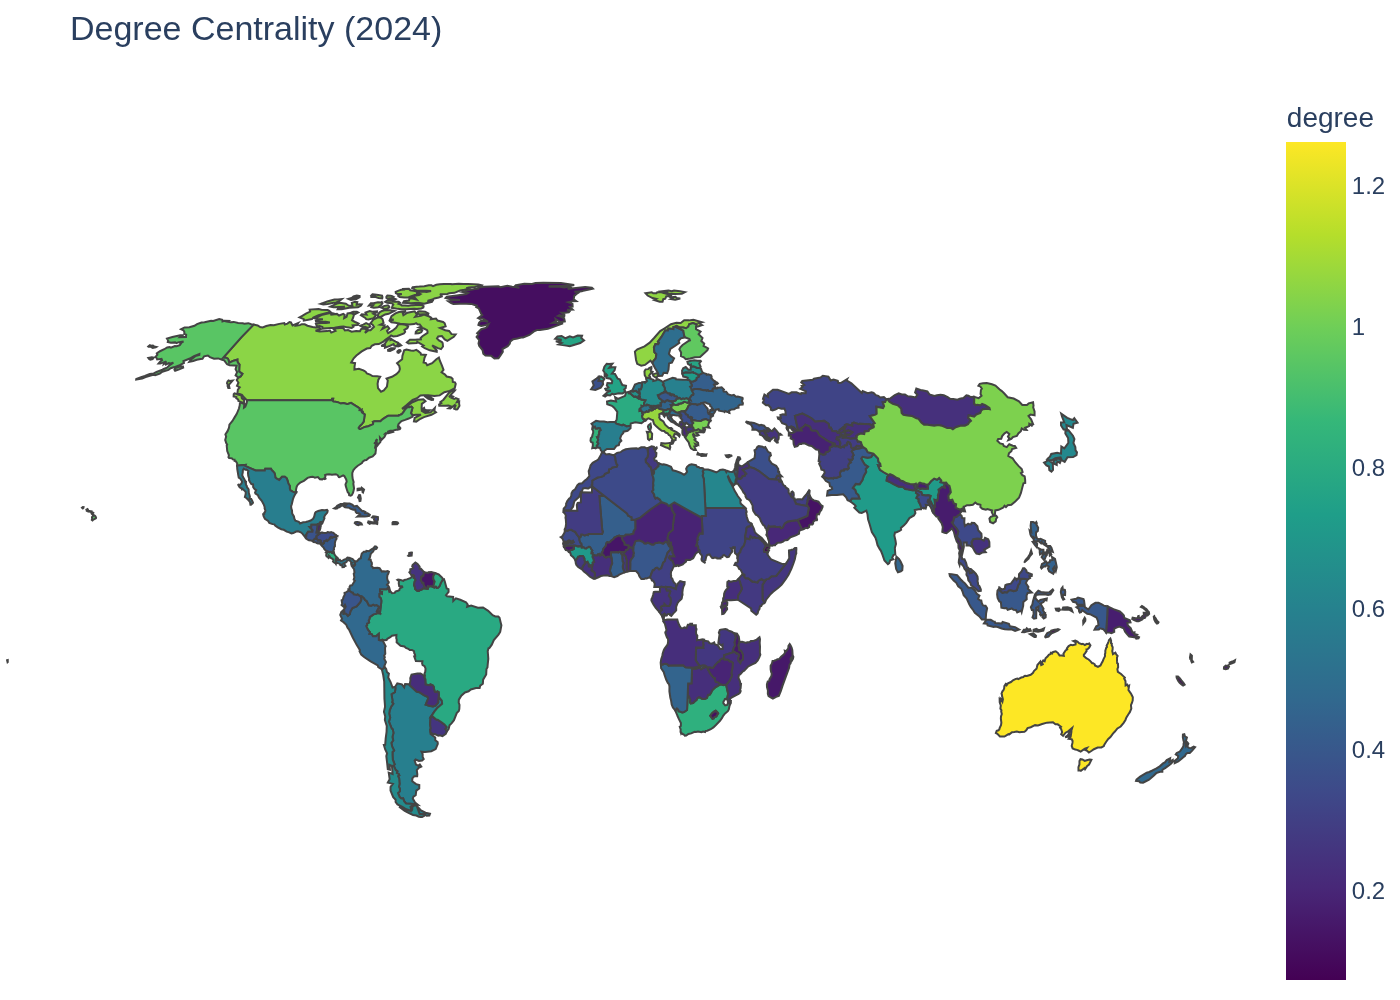
\includegraphics[width=0.9\textwidth]{deliverables_outputs/visuals/map_degree.png}
  \caption{Degree centrality map (2024). Countries with broad bilateral connectivity are highlighted.}
\end{figure}
\noindent\textit{Explanation:} Degree centrality measures the number of direct migration connections. High values indicate countries connected to many origins or destinations, reflecting breadth of links rather than depth of flows. In migration context, this highlights countries with diversified corridors and extensive global ties.

\section{Betweenness Centrality}
\begin{figure}[H]
  \centering
  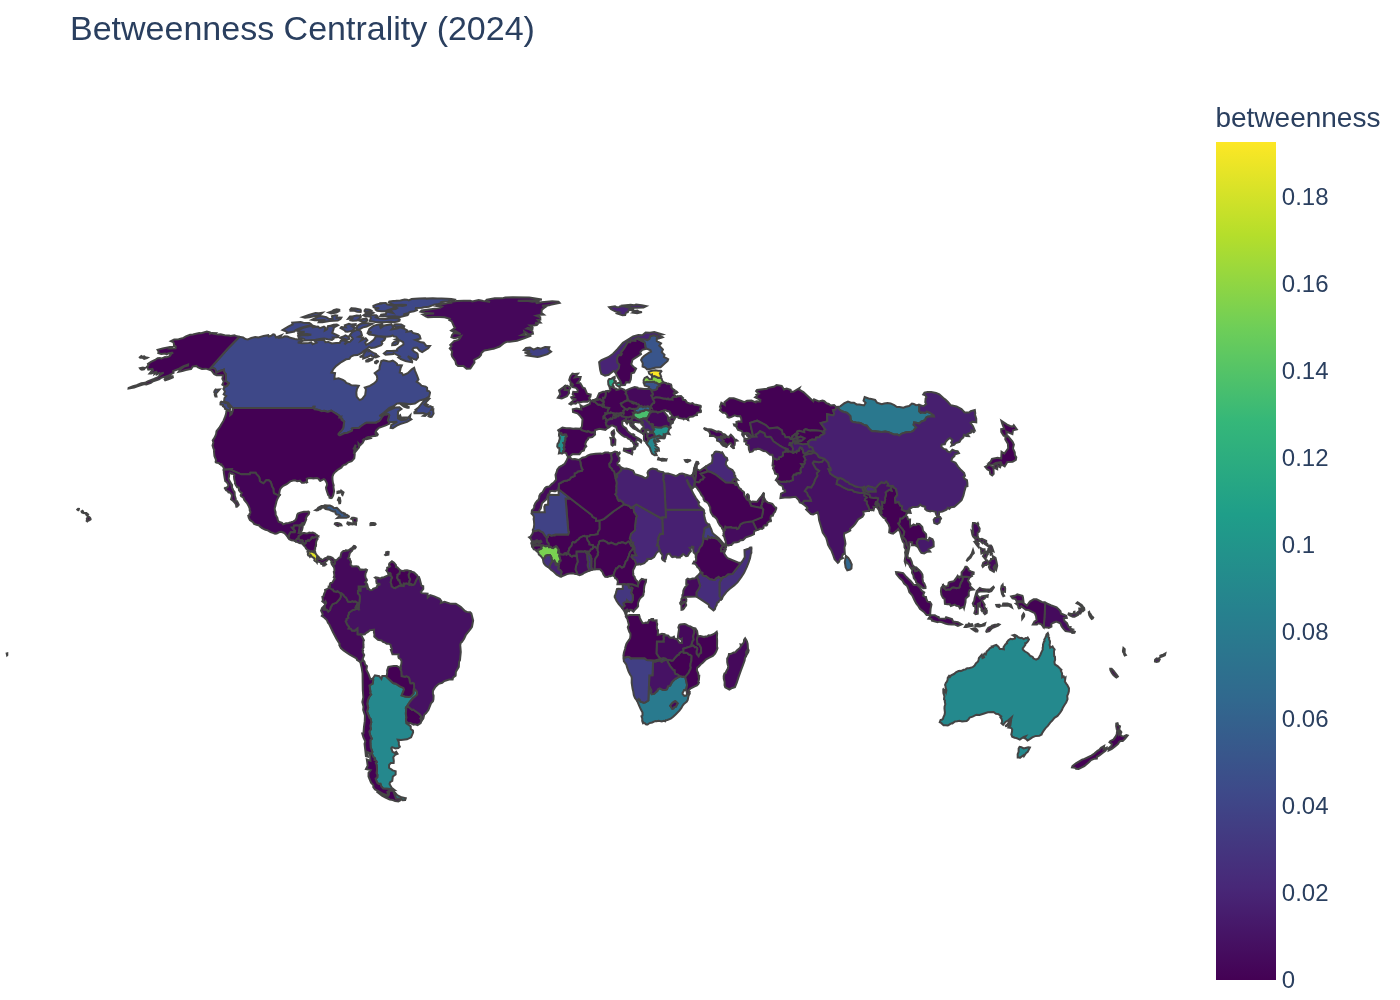
\includegraphics[width=0.9\textwidth]{deliverables_outputs/visuals/map_betweenness.png}
  \caption{Betweenness centrality map (2024). Bridge countries between regions stand out.}
\end{figure}
\noindent\textit{Explanation:} Betweenness captures how often a country lies on shortest paths between other countries. High values indicate transit or bridge roles that connect regional blocs. These countries are strategically important because disruptions here can affect multiple corridors.

\section{Closeness Centrality}
\begin{figure}[H]
  \centering
  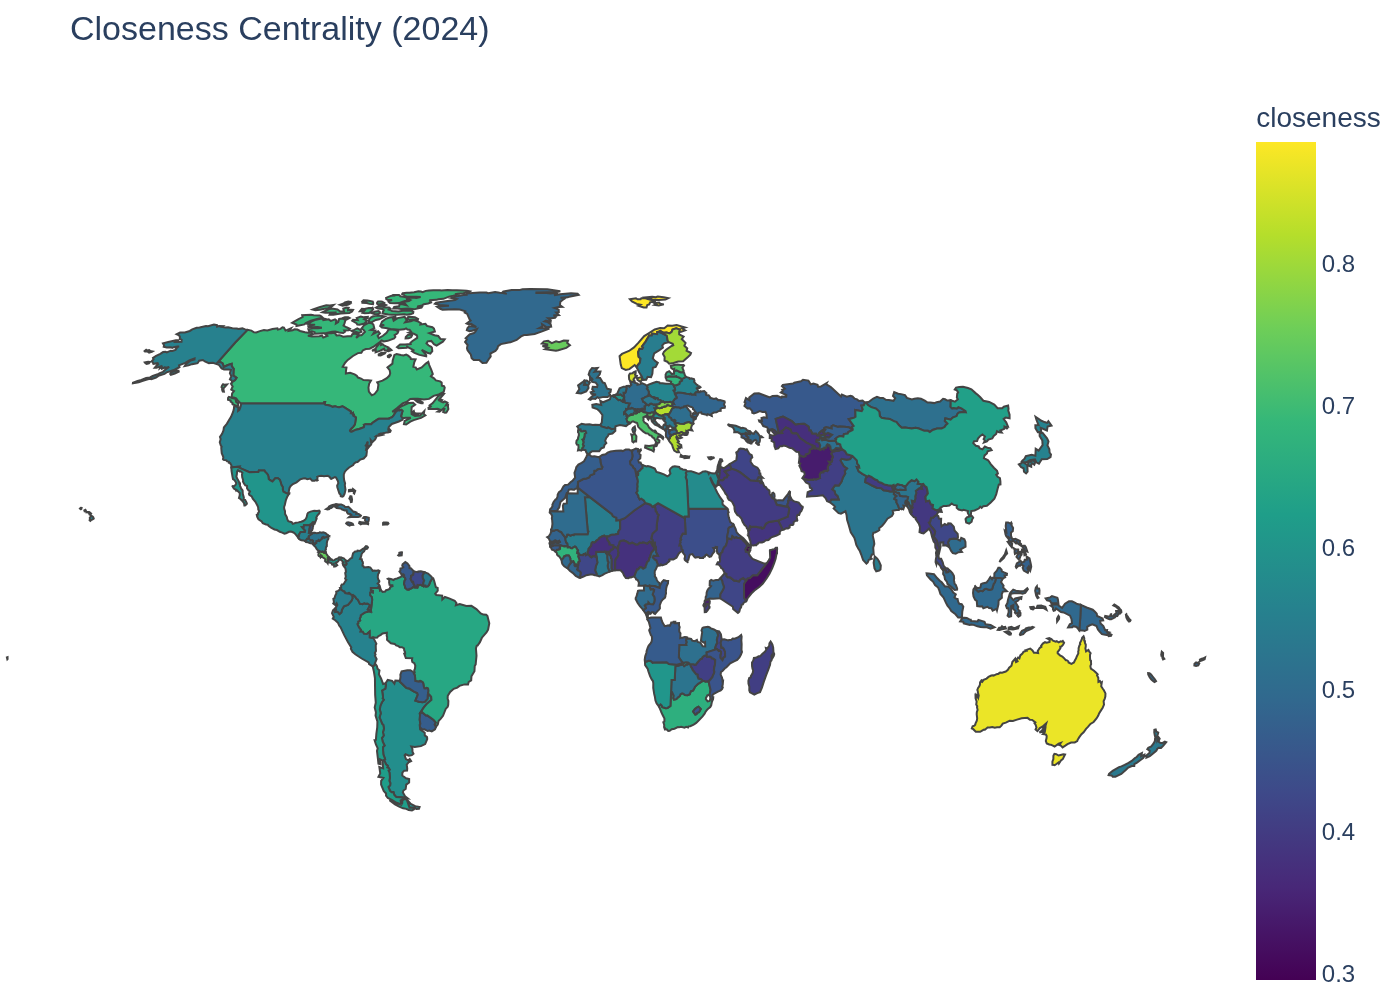
\includegraphics[width=0.9\textwidth]{deliverables_outputs/visuals/map_closeness.png}
  \caption{Closeness centrality map (2024). Centrally positioned countries appear with higher values.}
\end{figure}
\noindent\textit{Explanation:} Closeness centrality measures how quickly a country can reach all others in the network. In migration terms, high closeness suggests structural accessibility and efficient reachability from many regions. This indicates a globally central position even when flows are moderate.

\section{PageRank Centrality}
\begin{figure}[H]
  \centering
  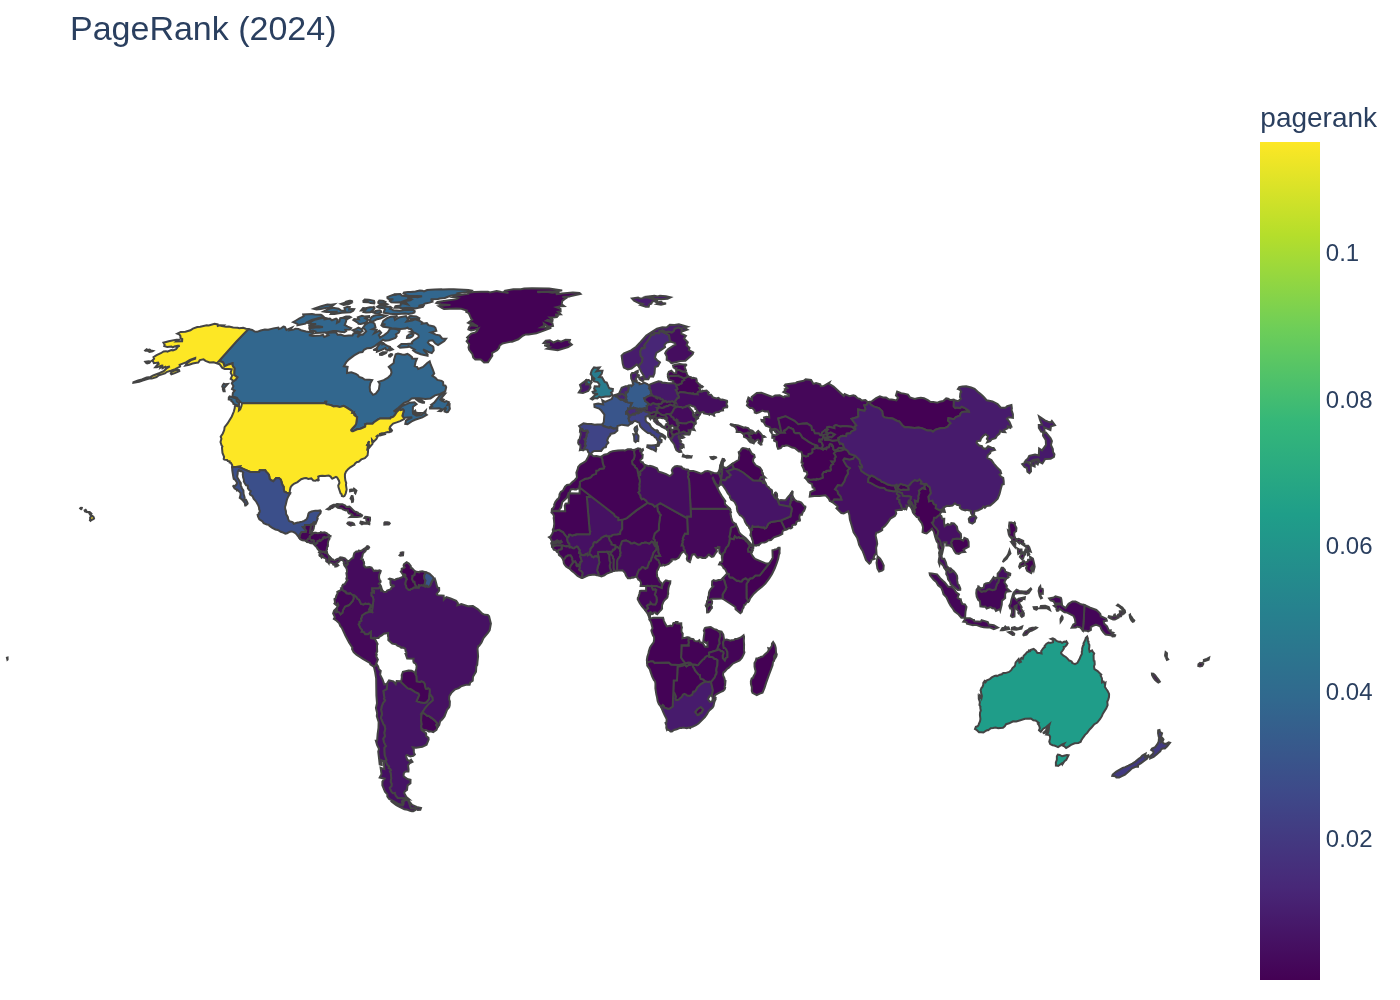
\includegraphics[width=0.9\textwidth]{deliverables_outputs/visuals/map_pagerank.png}
  \caption{PageRank map (2024). Globally influential migration hubs are emphasized.}
\end{figure}
\noindent\textit{Explanation:} PageRank rewards links from other influential countries, capturing global influence instead of simple connectivity. High PageRank countries are durable hubs with strong indirect influence. This differentiates major global destinations from locally connected nodes.

\section{Network Visualization (Community Structure)}
\begin{figure}[H]
  \centering
  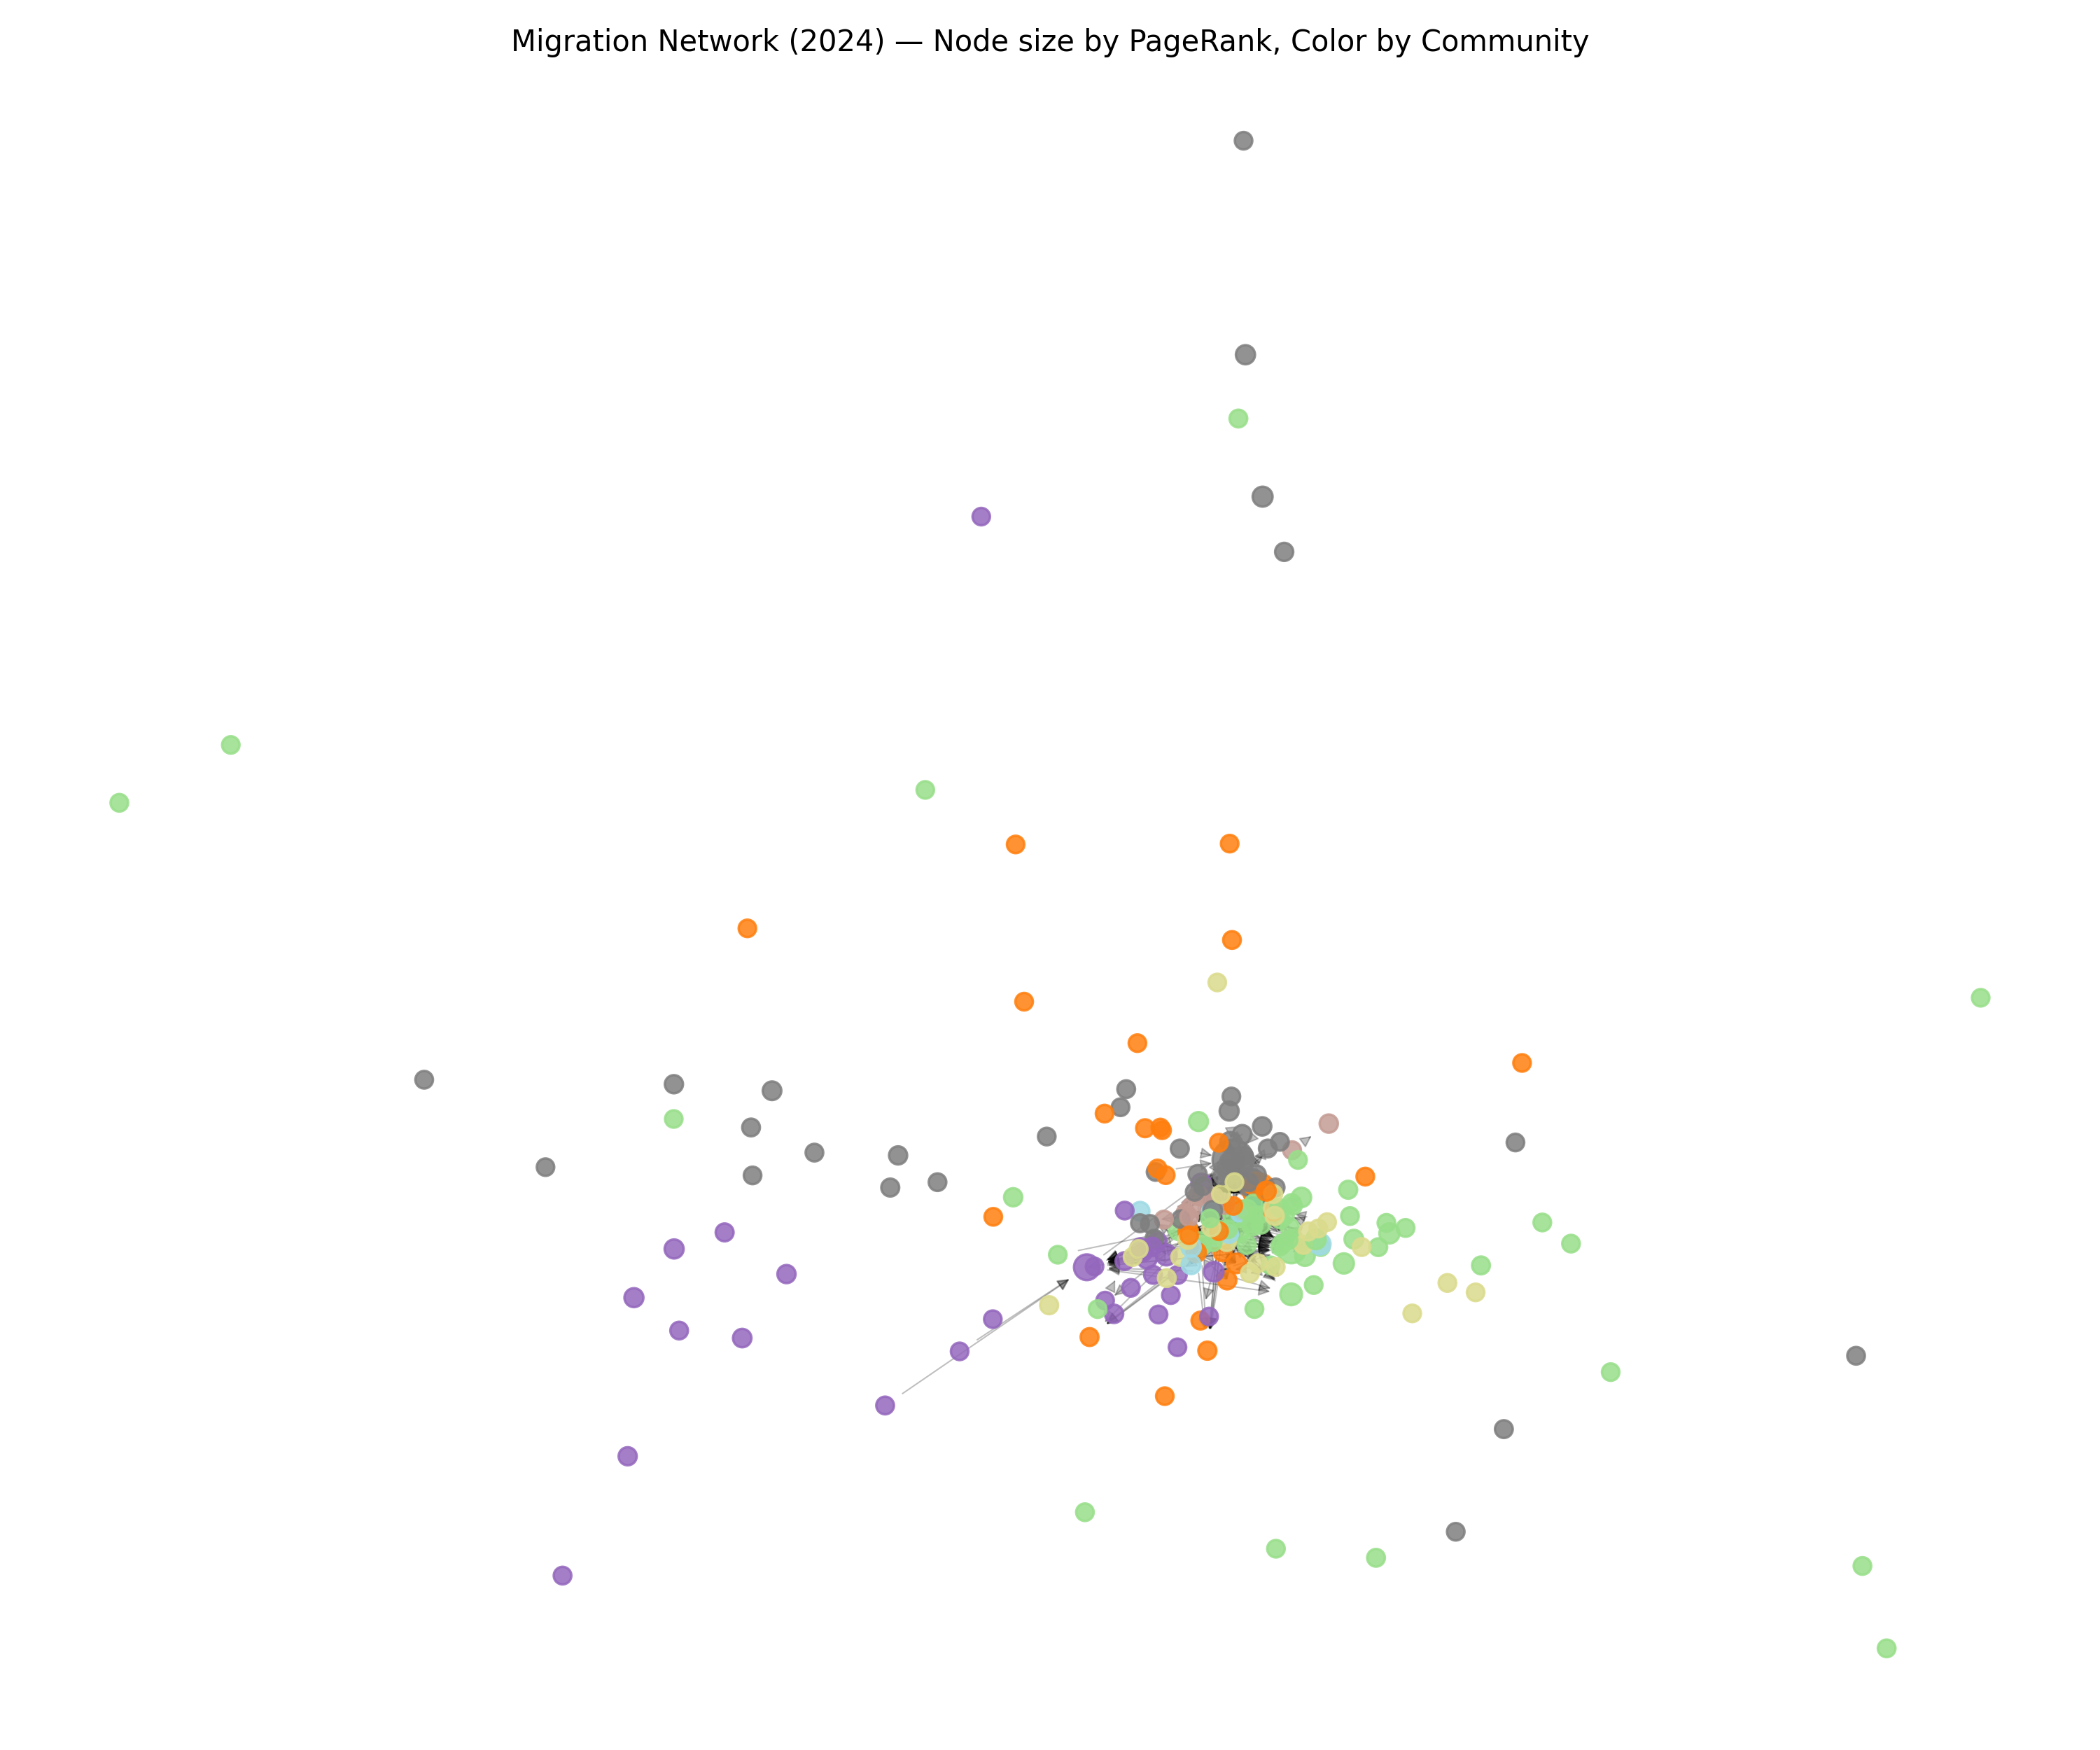
\includegraphics[width=0.9\textwidth]{deliverables_outputs/visuals/network_pagerank_community.png}
  \caption{Migration network (2024) with node size proportional to PageRank and node color by community.}
\end{figure}
\noindent\textit{Explanation:} Node size highlights global influence, while colors show community membership. The visualization reveals clustered regional blocs and a few dominant hubs, consistent with scale-free structure and persistent migration cores.

\chapter{Case Study: Syria $\rightarrow$ T\"urkiye}
This corridor illustrates conflict-driven migration and shifting community membership. T\"urkiye acts as a regional bridge with high betweenness, linking origin regions to European destinations.

\chapter{Visual Outputs}
\section{5-Year Interval Visualizations}
\begin{figure}[H]
  \centering
  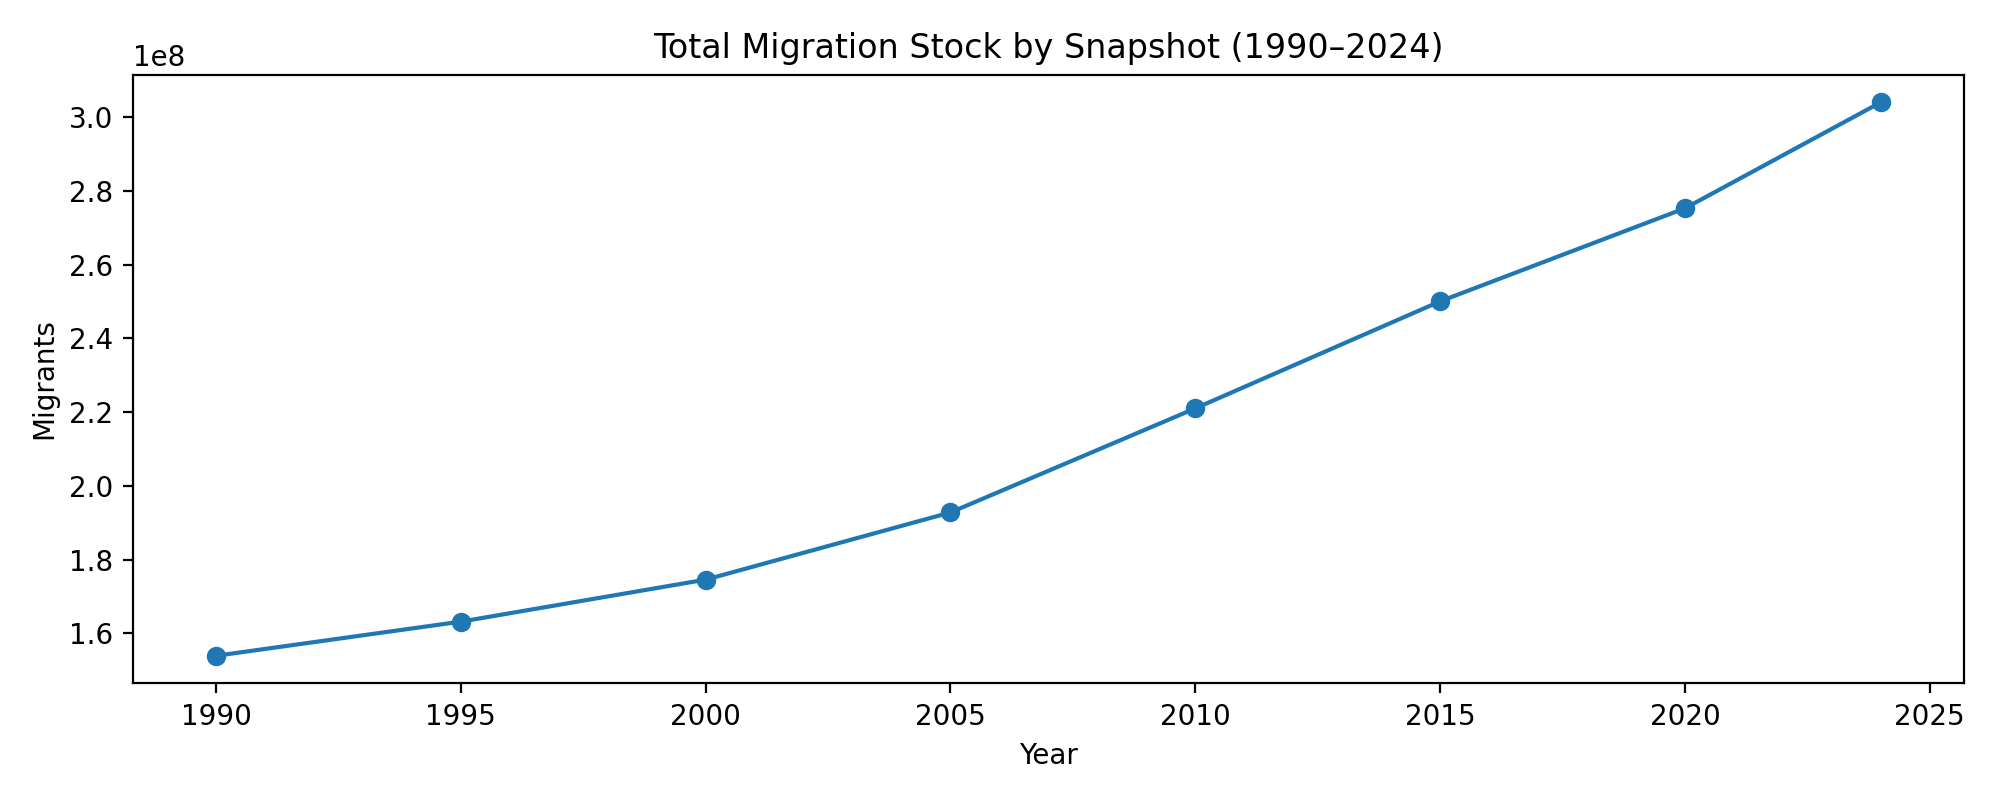
\includegraphics[width=0.9\textwidth]{deliverables_outputs/visuals/interval_total_trend.png}
  \caption{Total migration stock across snapshots (1990–2024).}
\end{figure}
\noindent\textit{Explanation:} This trend line captures the long-run growth in global migration stocks. The steady rise indicates structural persistence and cumulative migration effects over decades.

\begin{figure}[H]
  \centering
  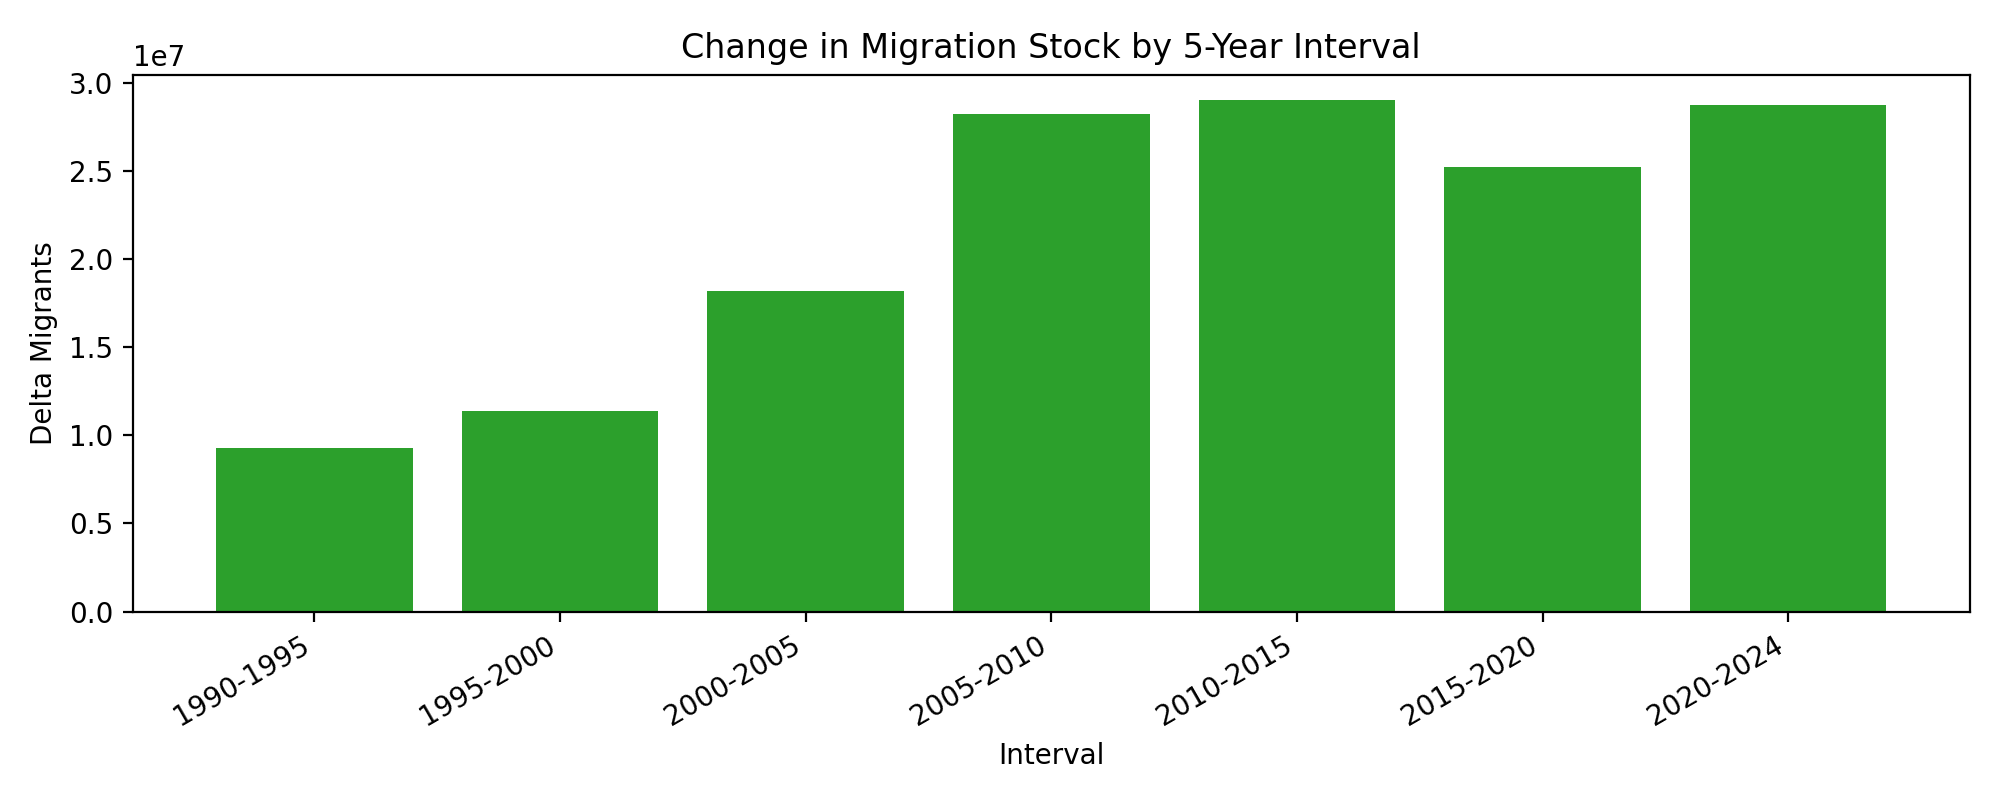
\includegraphics[width=0.9\textwidth]{deliverables_outputs/visuals/interval_delta_bar.png}
  \caption{Change in migration stock by 5-year interval.}
\end{figure}
\noindent\textit{Explanation:} Each bar shows the absolute change between consecutive snapshots (1990–1995, 1995–2000, …, 2020–2024). Larger increases indicate periods of accelerated migration growth.

\section{Top Corridors per Interval}
\begin{figure}[H]
  \centering
  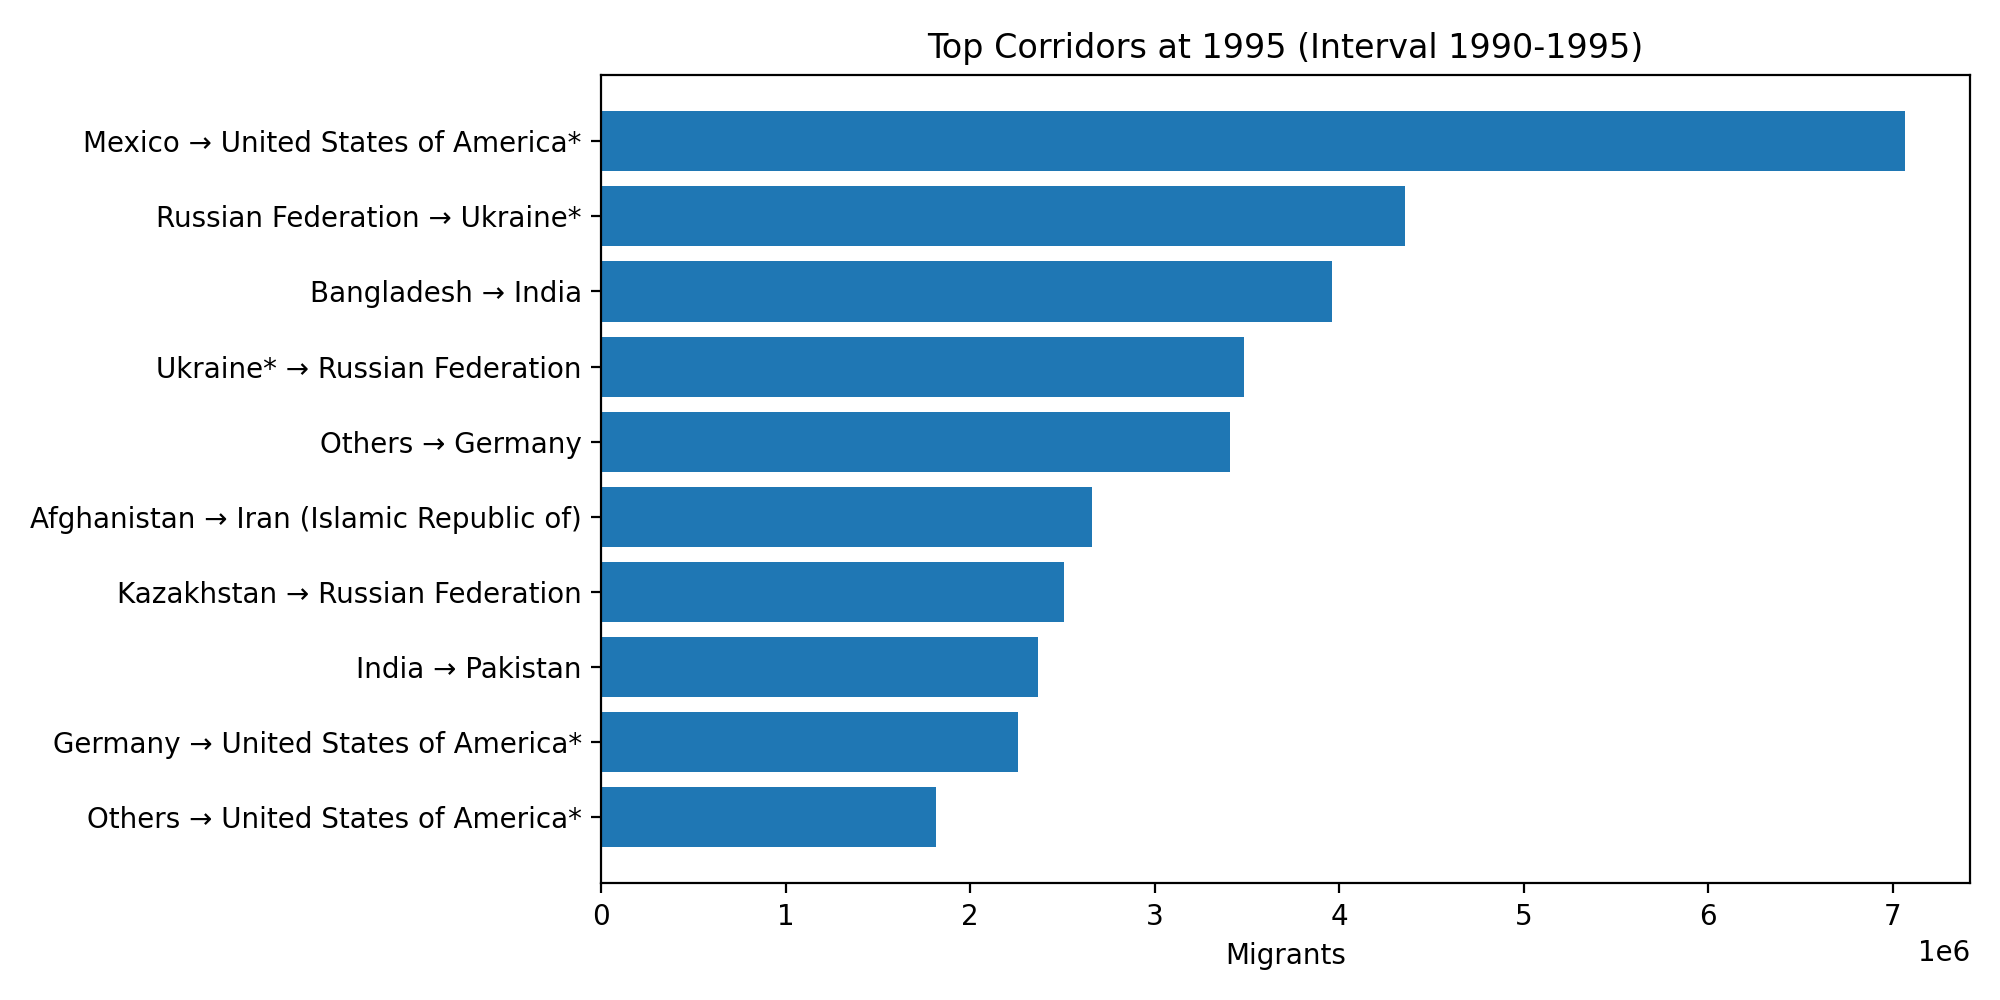
\includegraphics[width=0.9\textwidth]{deliverables_outputs/visuals/interval_top_corridors_1990_1995.png}
  \caption{Top corridors at 1995 (interval 1990–1995).}
\end{figure}
\begin{figure}[H]
  \centering
  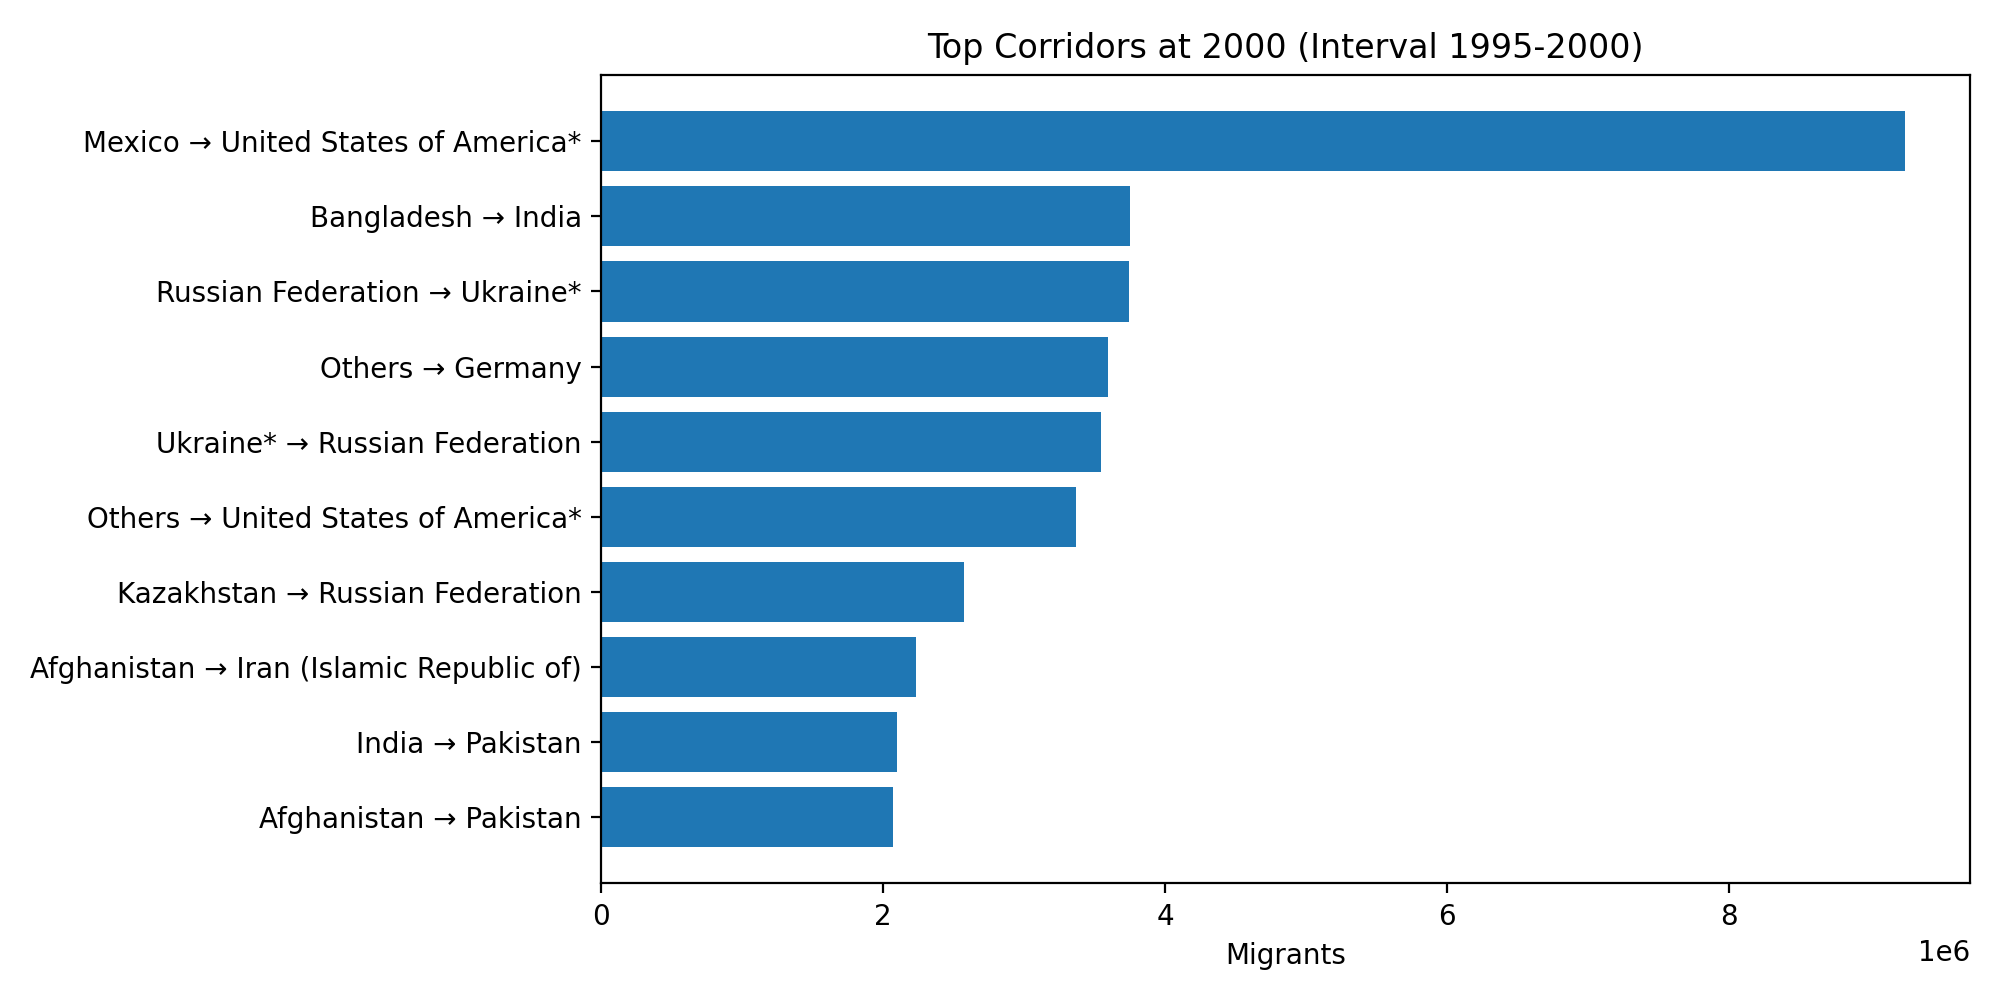
\includegraphics[width=0.9\textwidth]{deliverables_outputs/visuals/interval_top_corridors_1995_2000.png}
  \caption{Top corridors at 2000 (interval 1995–2000).}
\end{figure}
\begin{figure}[H]
  \centering
  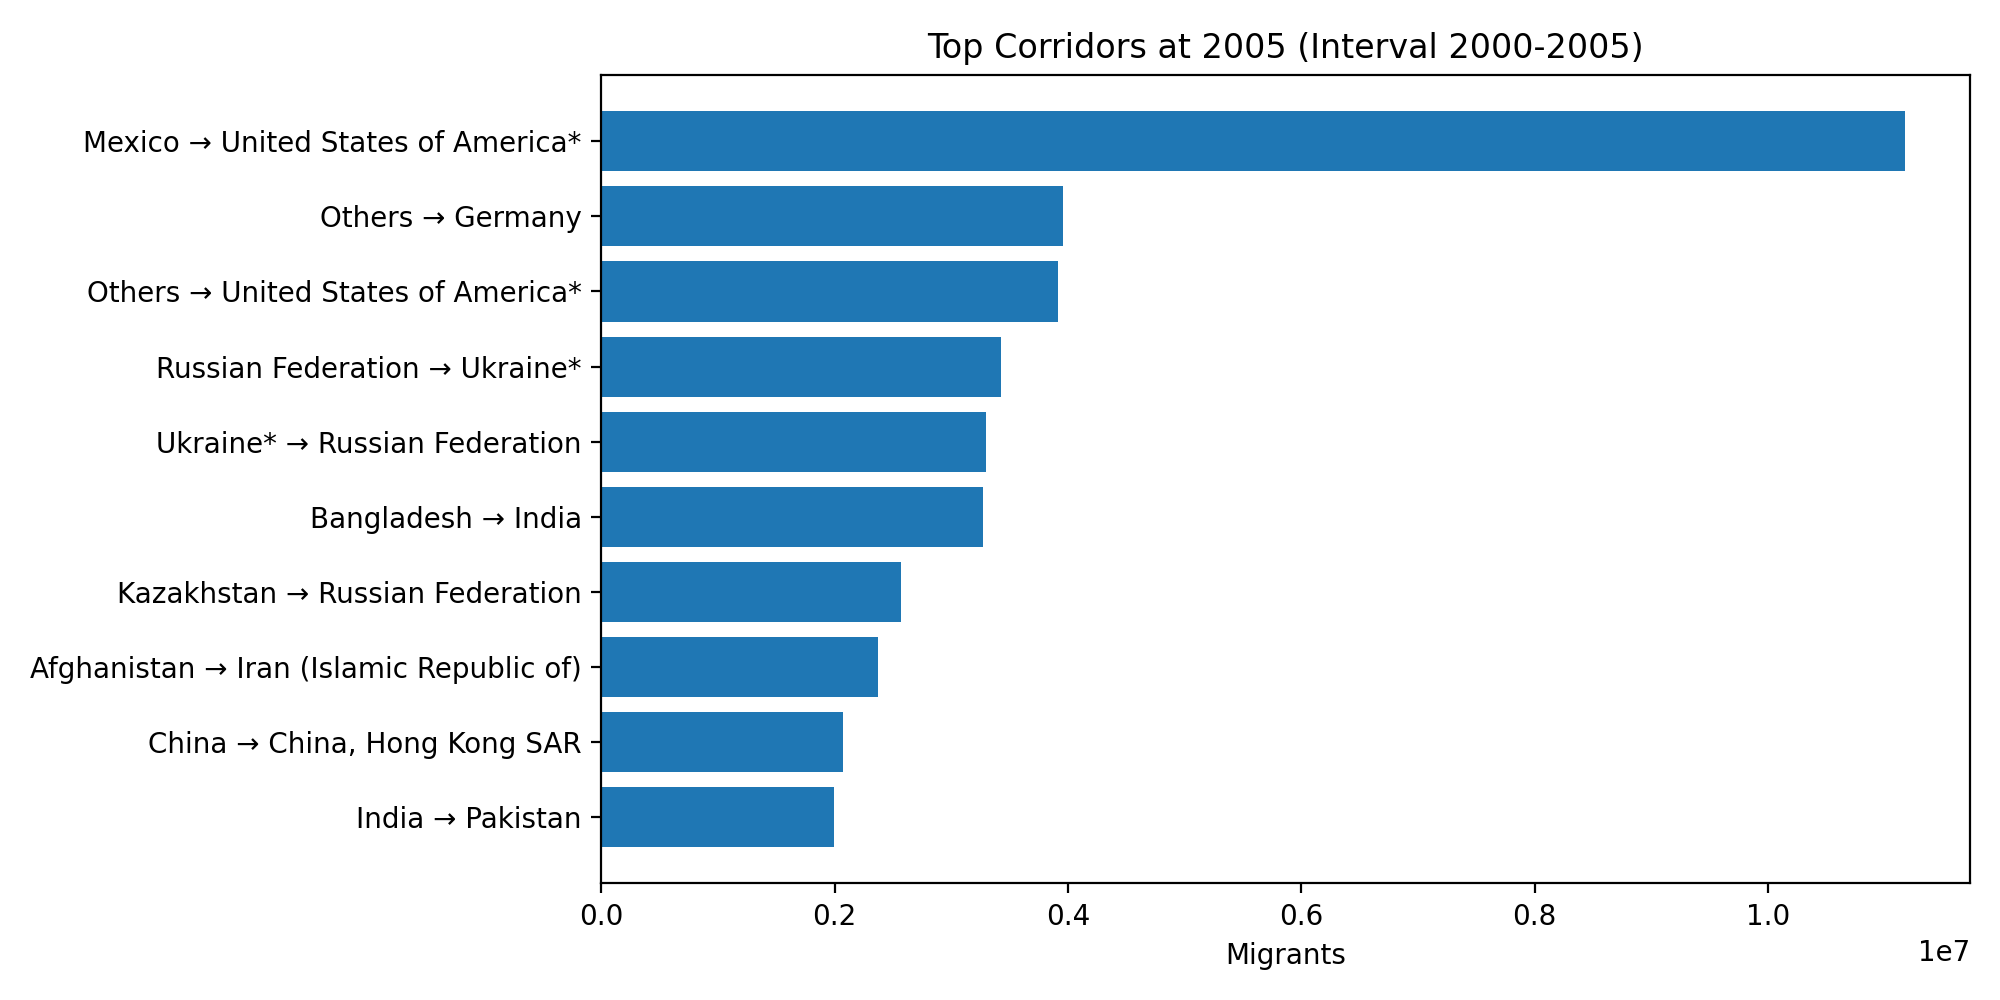
\includegraphics[width=0.9\textwidth]{deliverables_outputs/visuals/interval_top_corridors_2000_2005.png}
  \caption{Top corridors at 2005 (interval 2000–2005).}
\end{figure}
\begin{figure}[H]
  \centering
  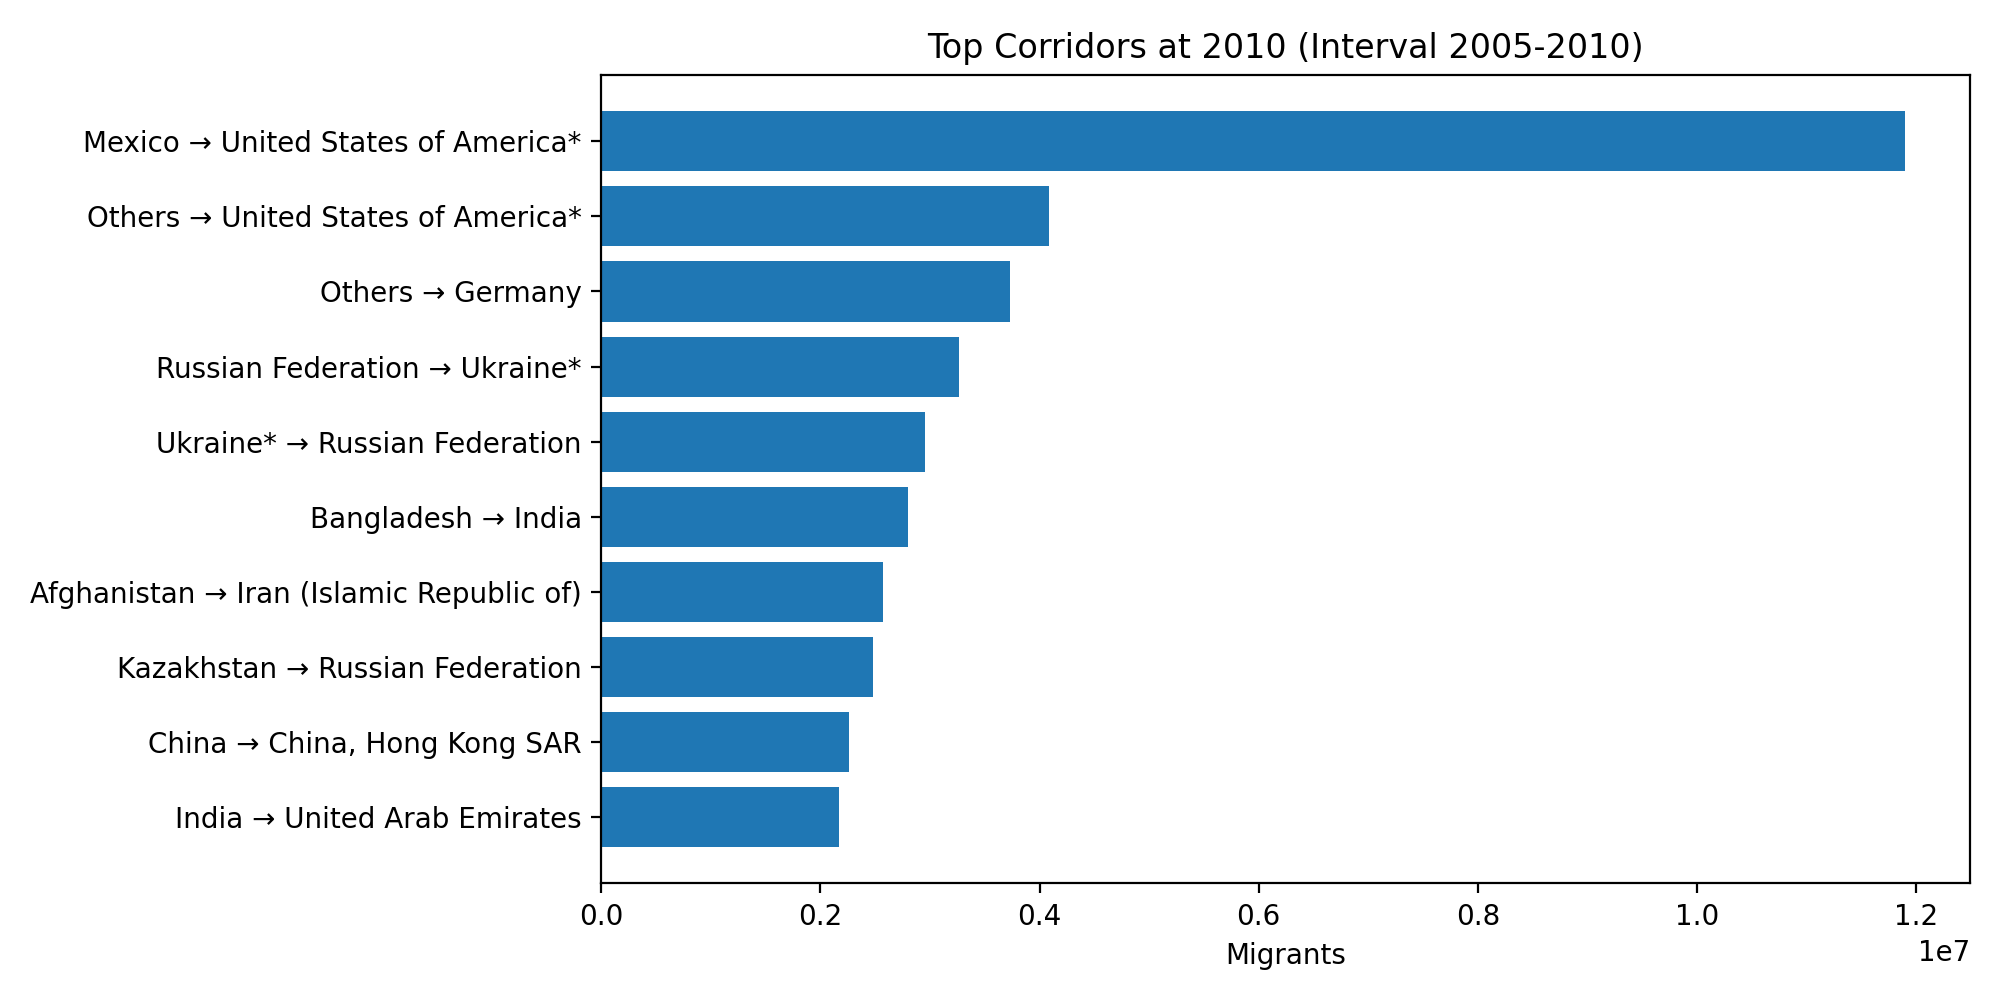
\includegraphics[width=0.9\textwidth]{deliverables_outputs/visuals/interval_top_corridors_2005_2010.png}
  \caption{Top corridors at 2010 (interval 2005–2010).}
\end{figure}
\begin{figure}[H]
  \centering
  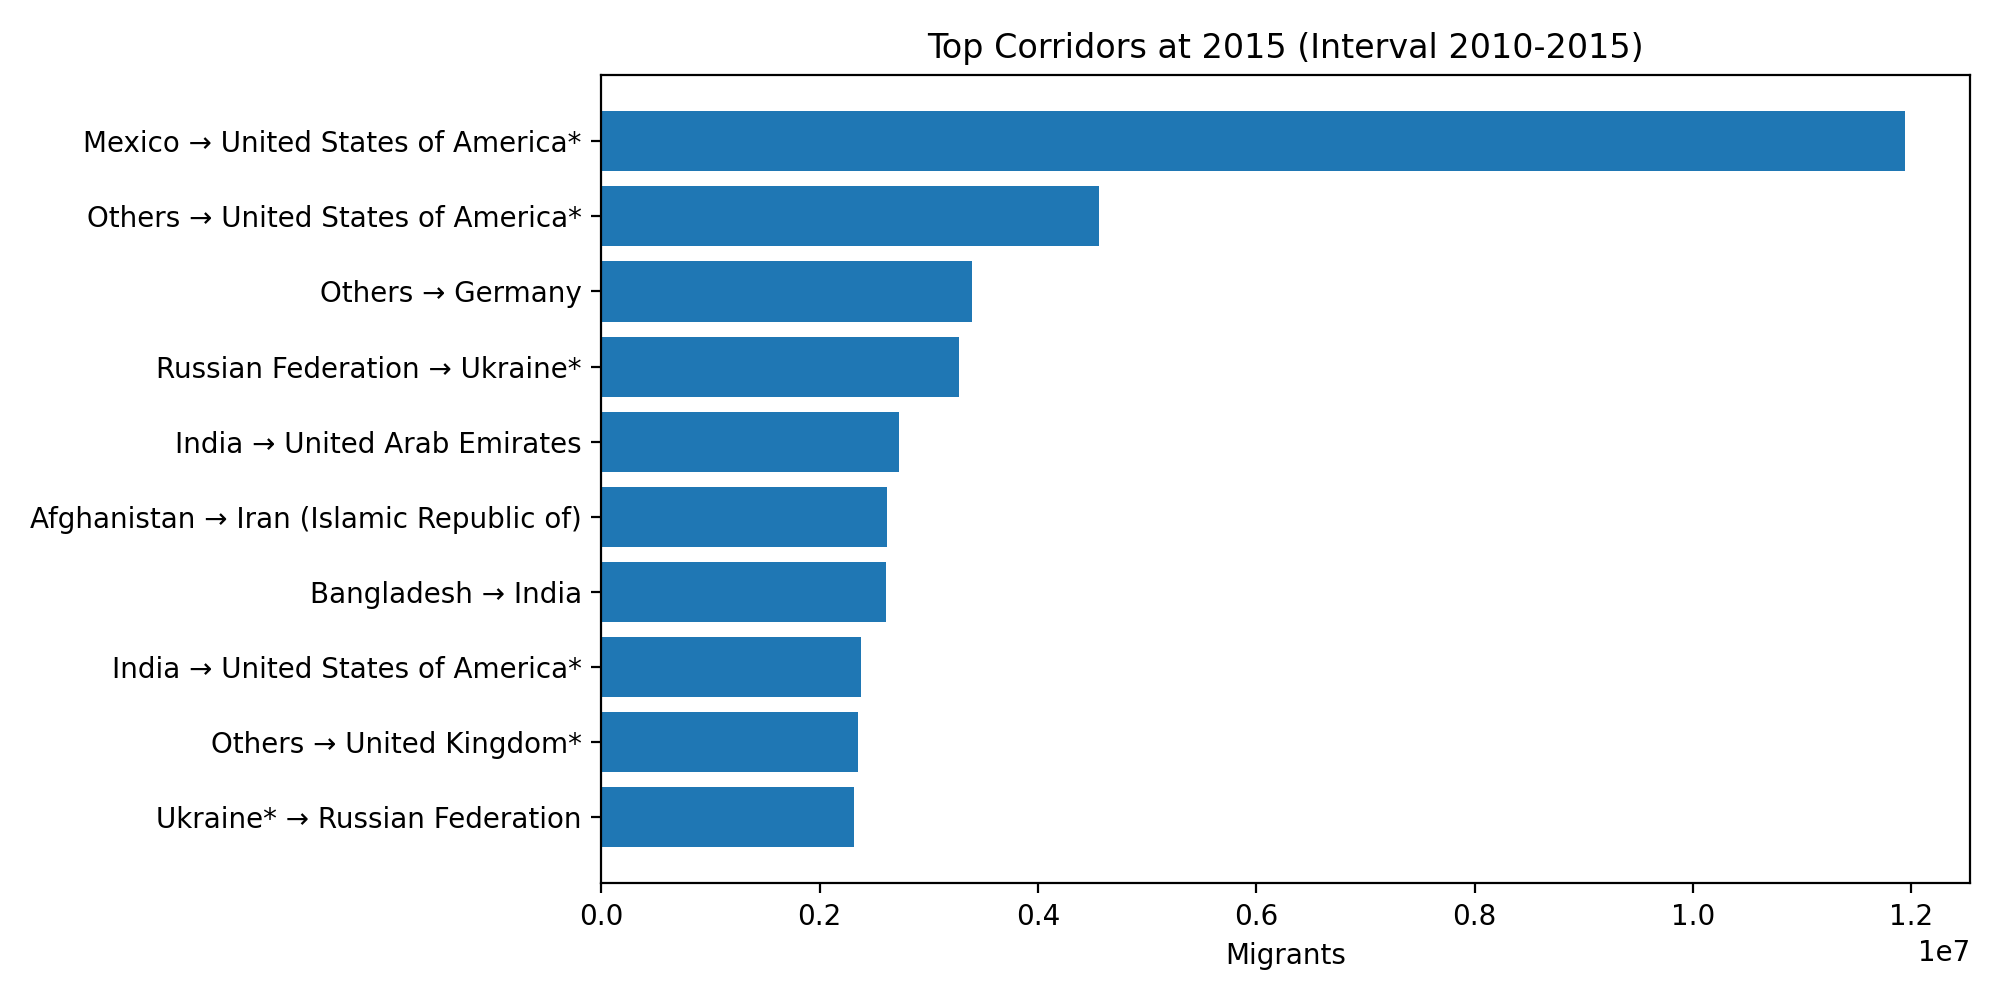
\includegraphics[width=0.9\textwidth]{deliverables_outputs/visuals/interval_top_corridors_2010_2015.png}
  \caption{Top corridors at 2015 (interval 2010–2015).}
\end{figure}
\begin{figure}[H]
  \centering
  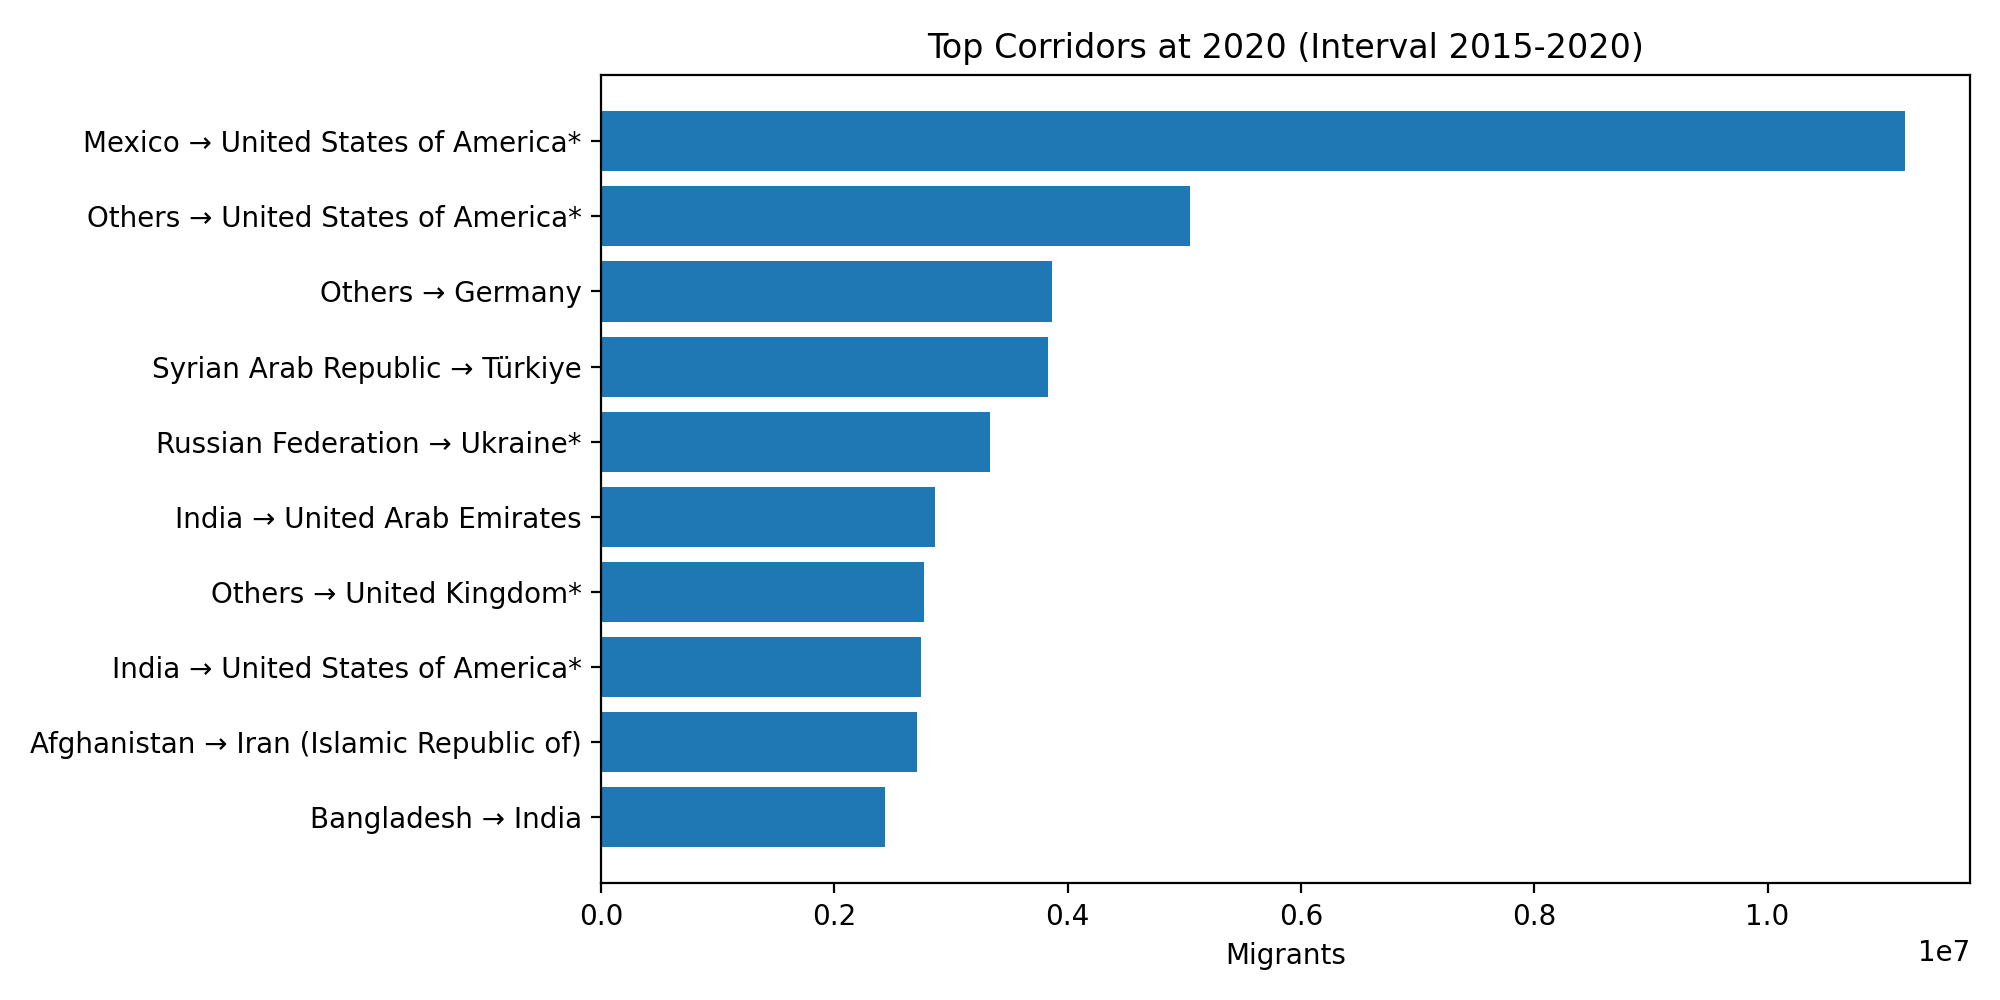
\includegraphics[width=0.9\textwidth]{deliverables_outputs/visuals/interval_top_corridors_2015_2020.png}
  \caption{Top corridors at 2020 (interval 2015–2020).}
\end{figure}
\begin{figure}[H]
  \centering
  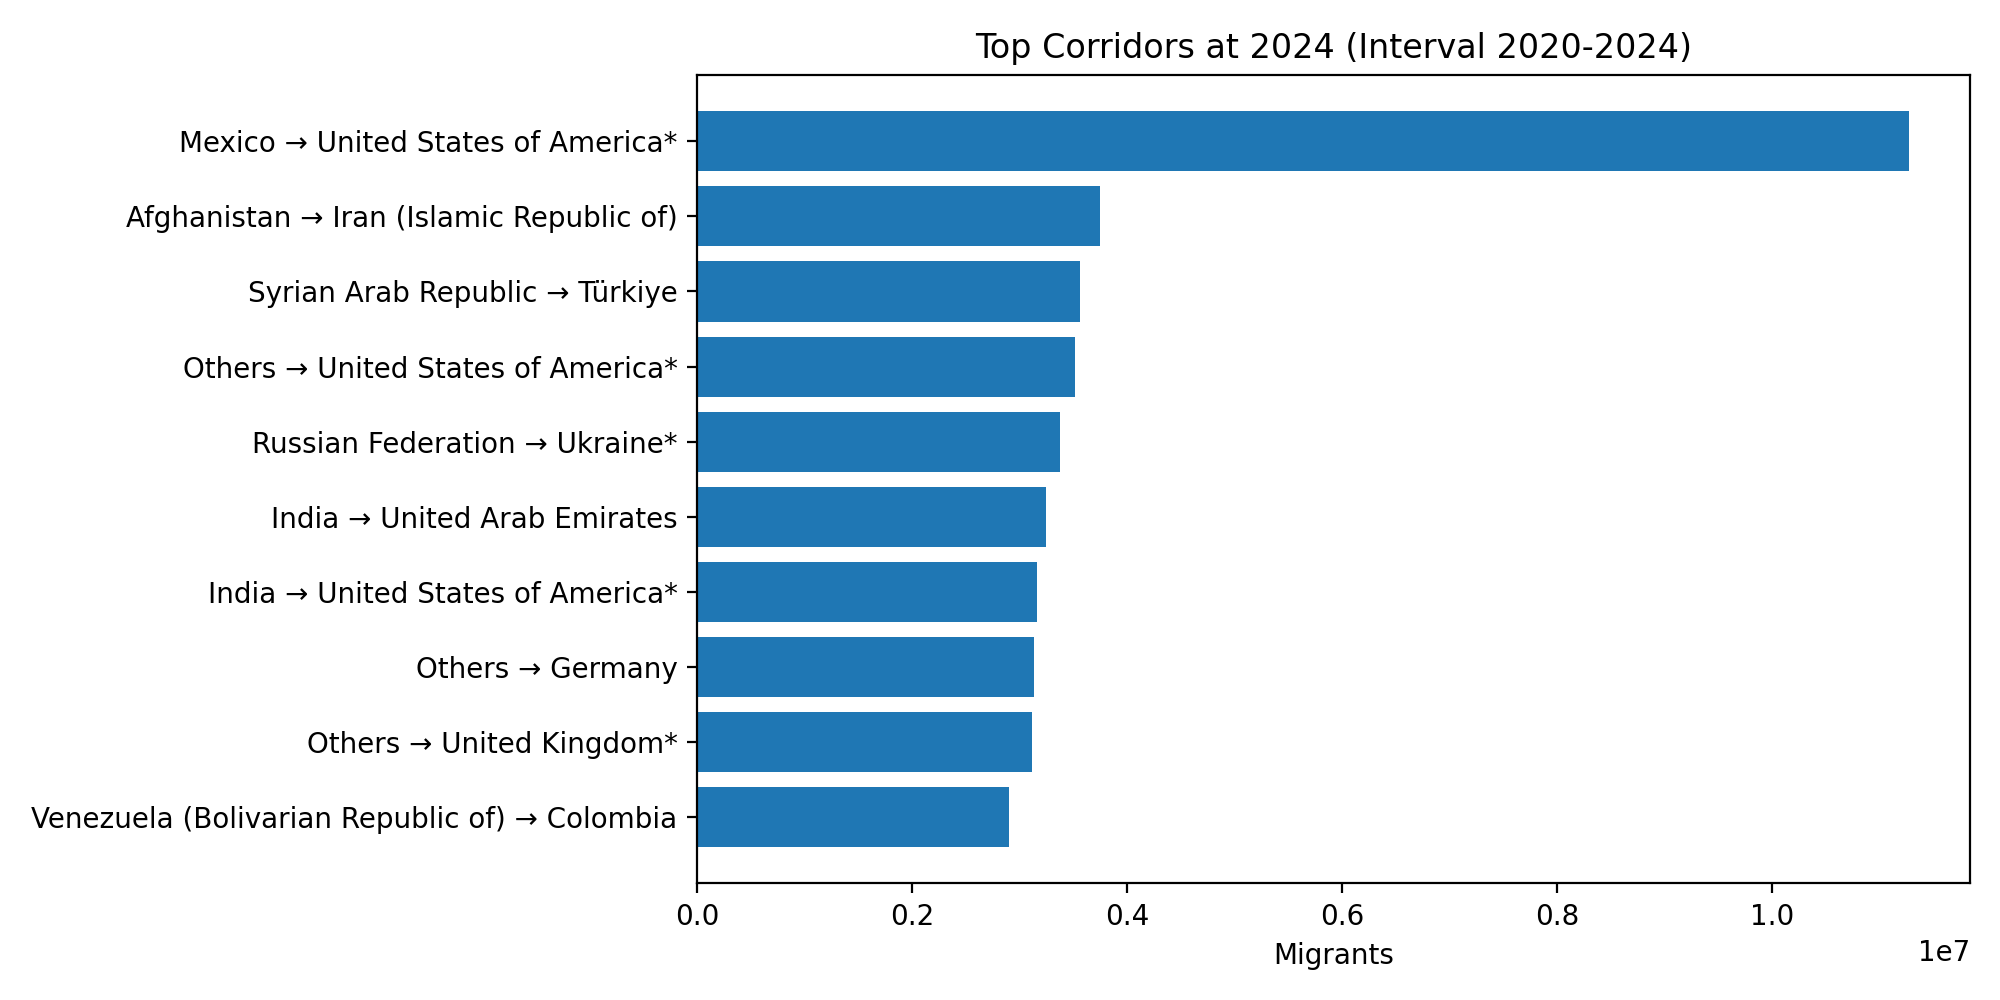
\includegraphics[width=0.9\textwidth]{deliverables_outputs/visuals/interval_top_corridors_2020_2024.png}
  \caption{Top corridors at 2024 (interval 2020–2024).}
\end{figure}
\noindent\textit{Explanation:} These panels show how leading corridors evolve by interval, highlighting persistent routes and emerging migration pathways.

\section{Final Collage (All Visuals Summary)}
\begin{figure}[H]
  \centering
  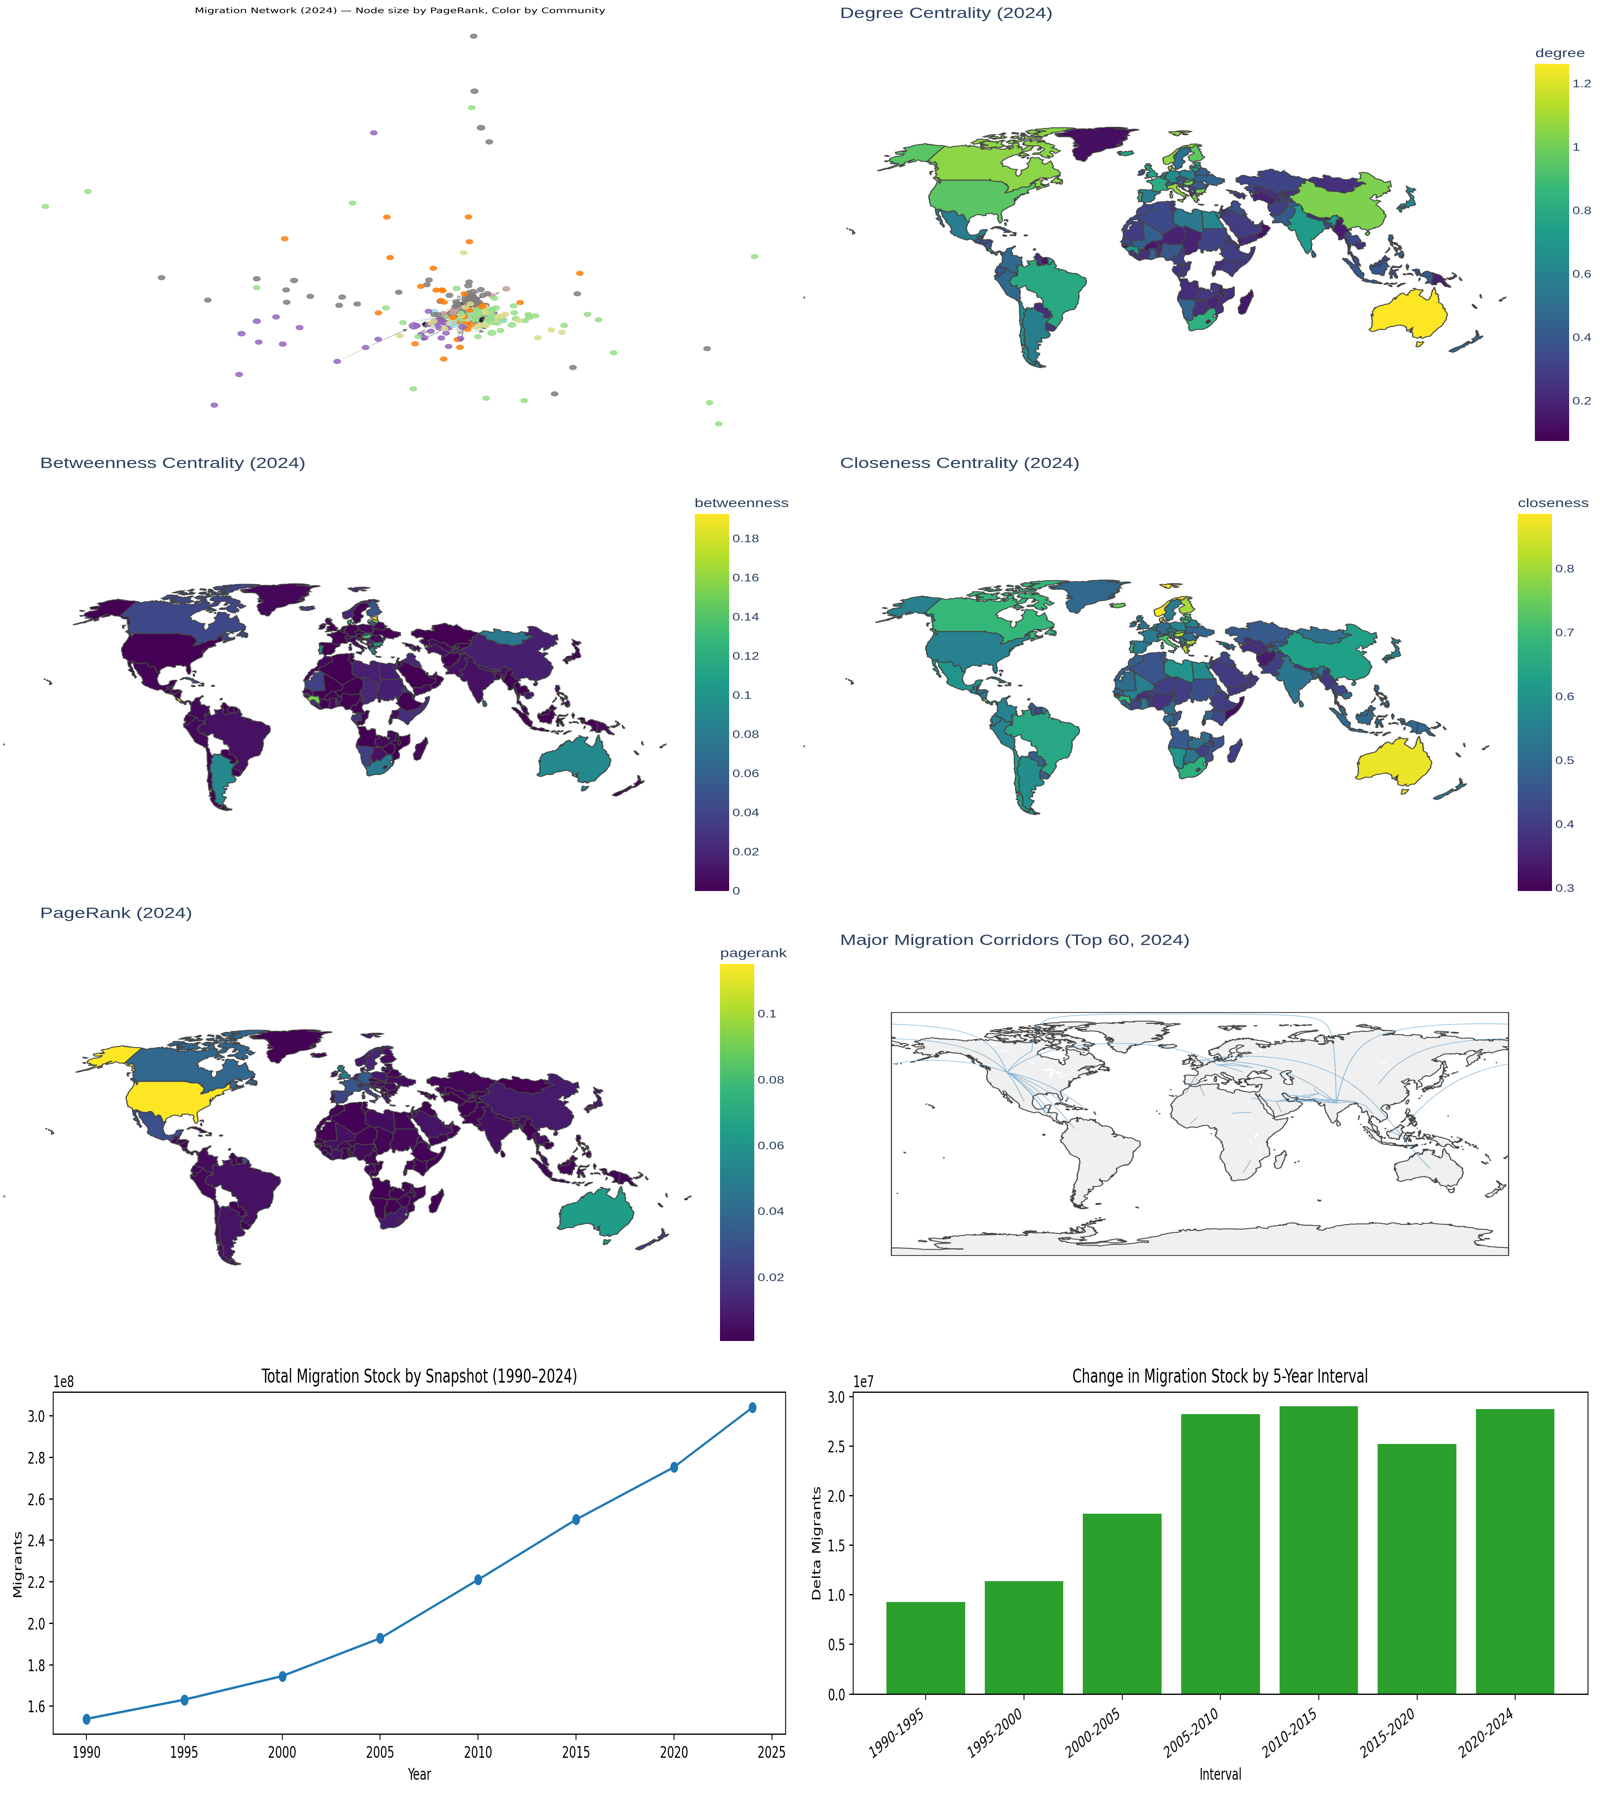
\includegraphics[width=0.95\textwidth]{deliverables_outputs/visuals/final_collage.png}
  \caption{Collage summary of key network, map, and interval visuals.}
\end{figure}
\noindent\textit{Explanation:} The collage provides a single-page visual overview of the project’s strongest plots, suitable for presentation and quick review.
\section{Major Corridors Map}
\begin{figure}[H]
  \centering
  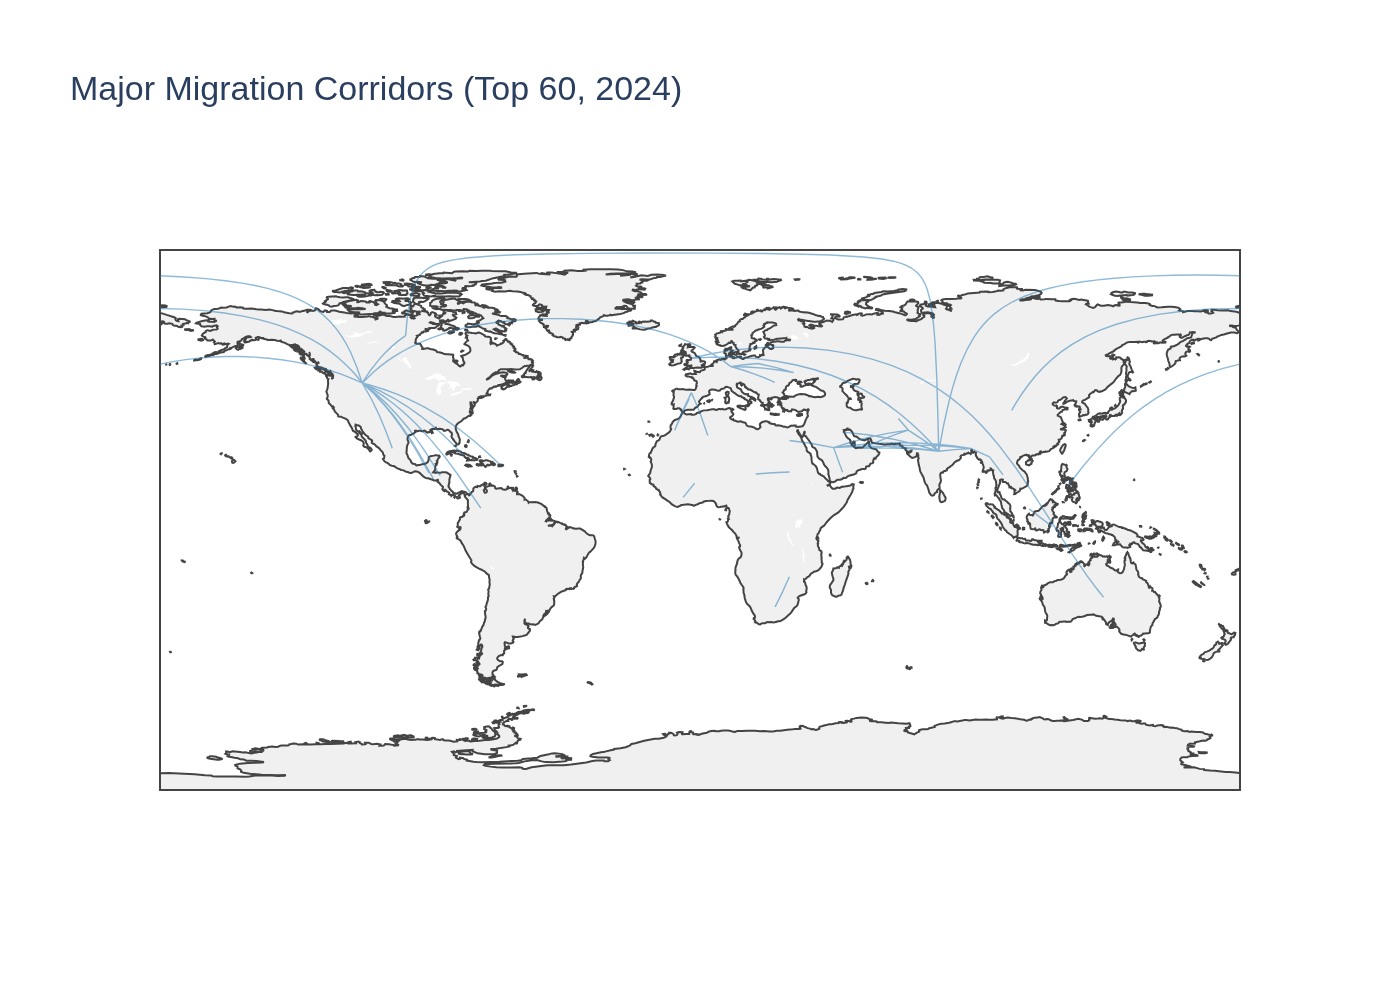
\includegraphics[width=0.9\textwidth]{deliverables_outputs/visuals/migration_corridors_map.png}
  \caption{Major migration corridors map (Top 60, 2024).}
\end{figure}
\noindent\textit{Explanation:} The most intense corridors reveal dominant origin--destination pathways. These flows reflect geopolitical, economic, and conflict-driven factors. The visualization shows strong regional concentration with a limited set of global super-corridors.

\section{Dashboard Screenshots}
\begin{figure}[H]
  \centering
  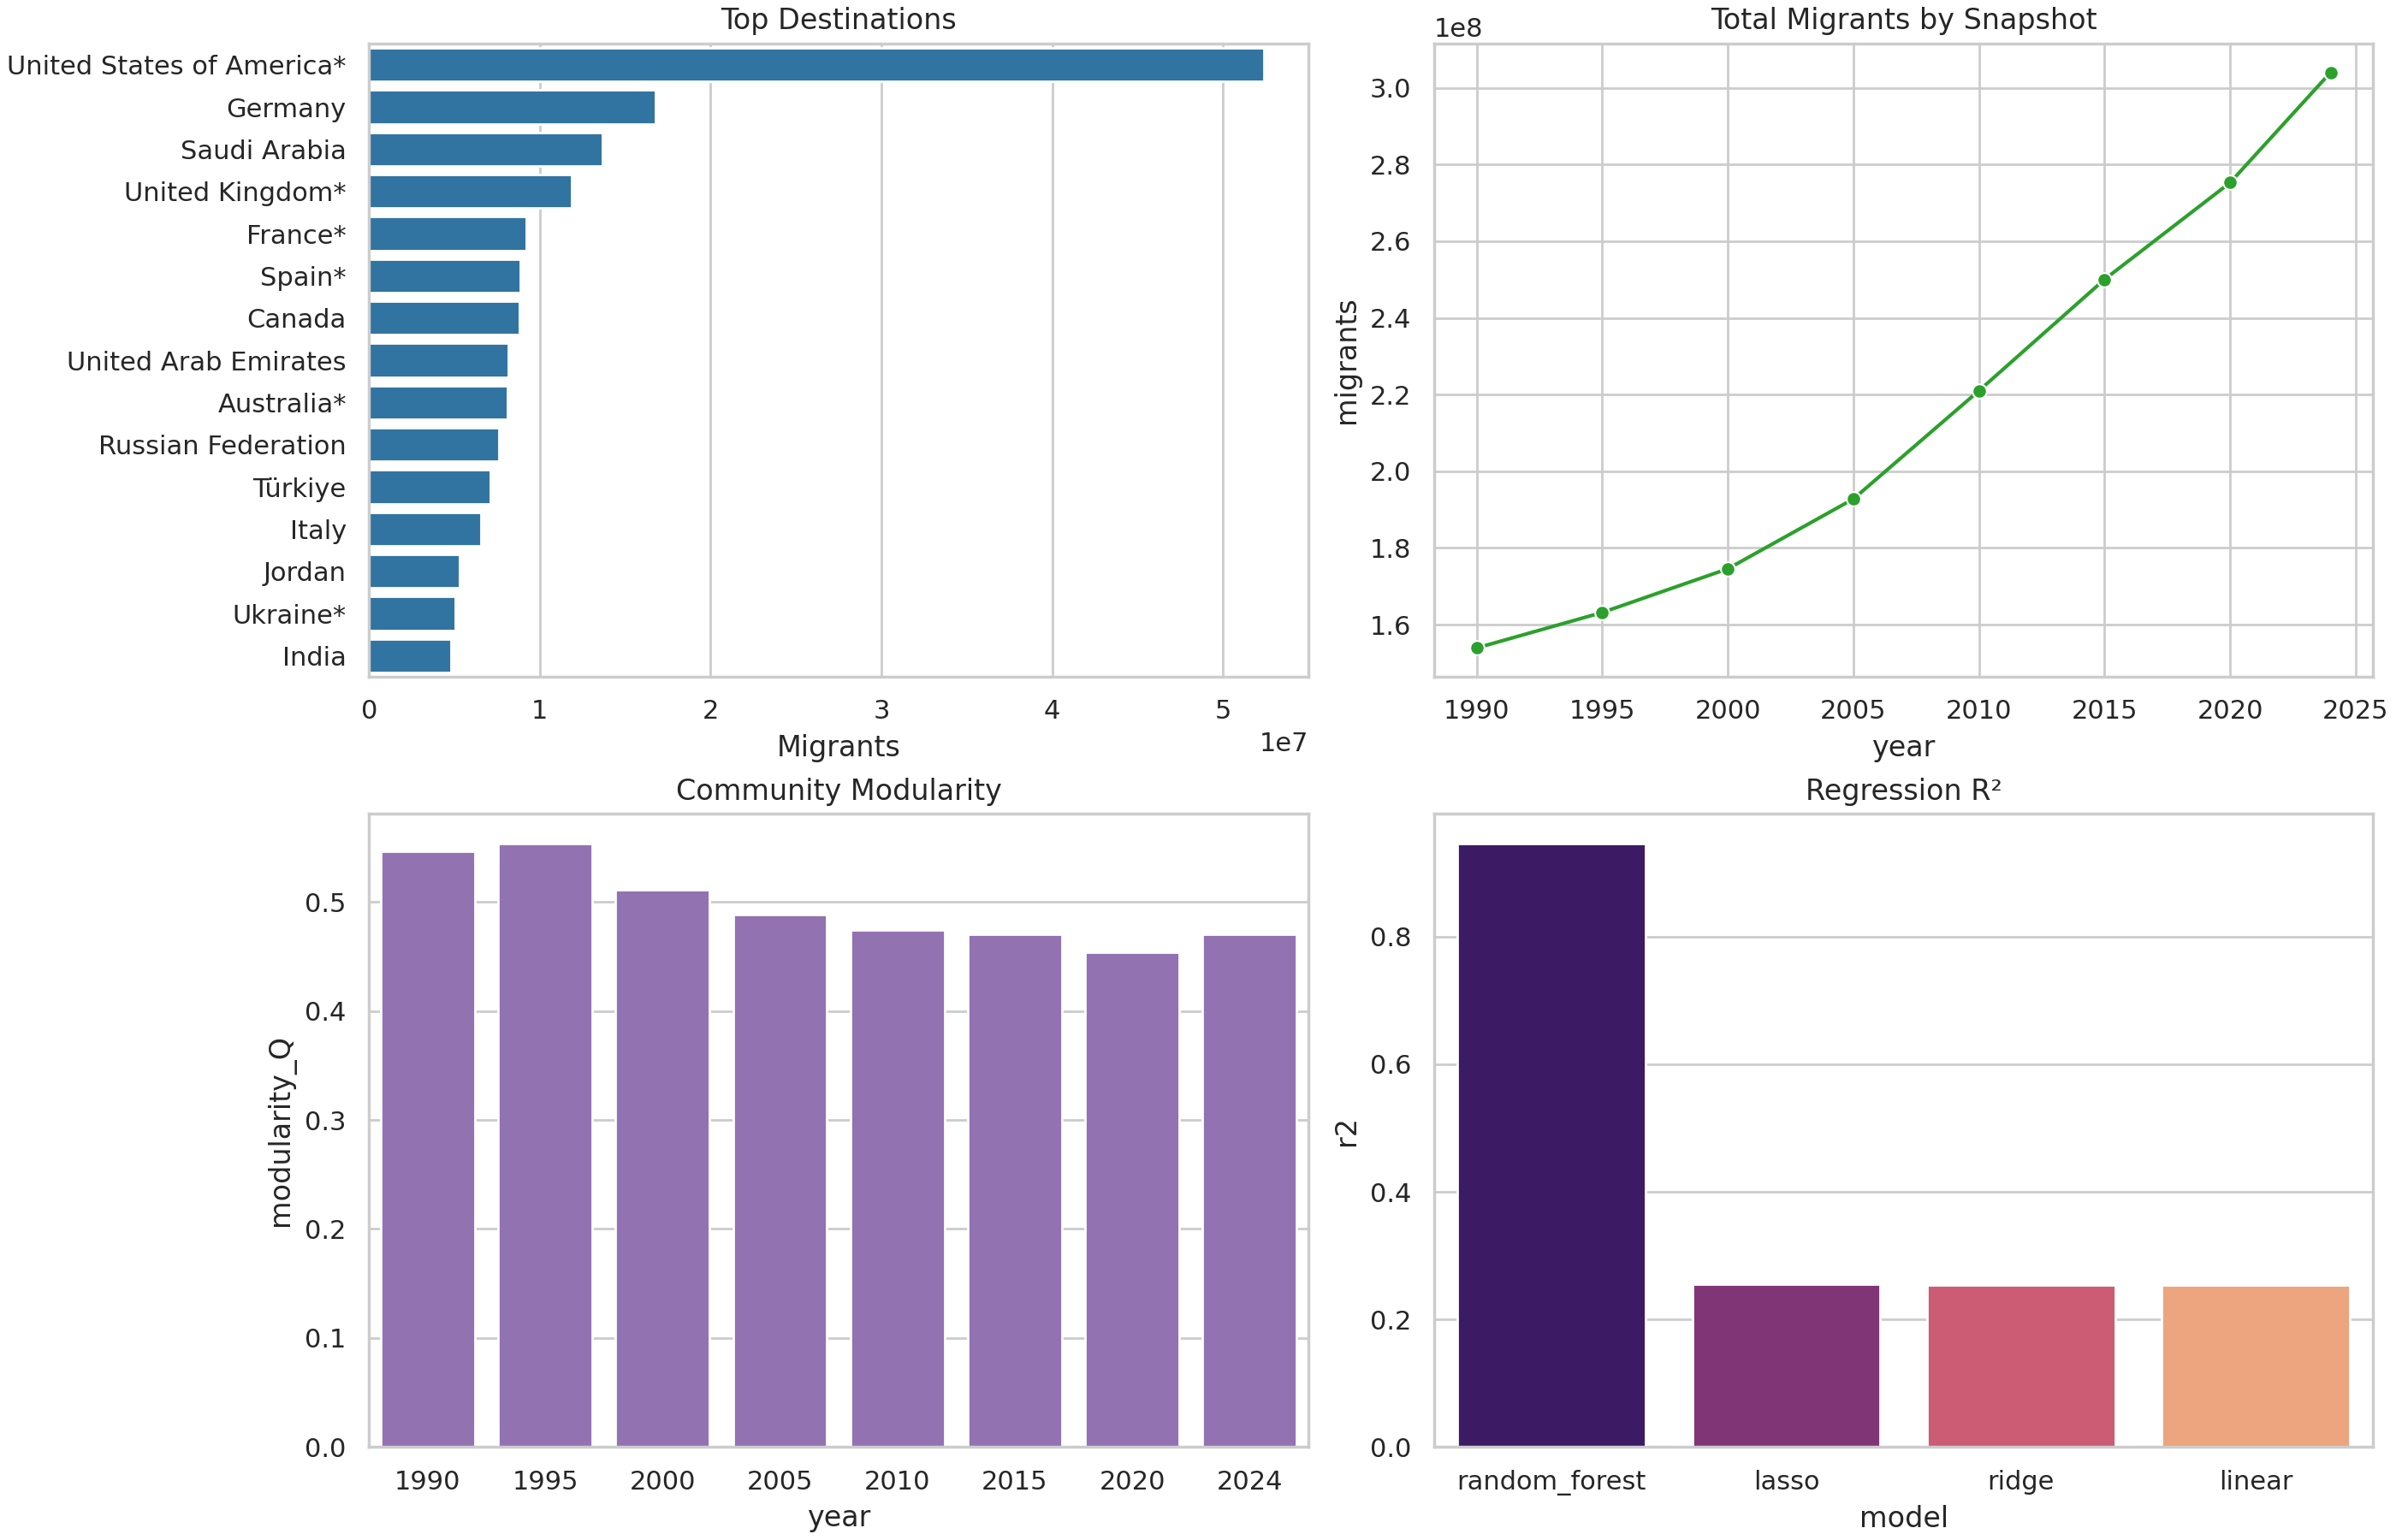
\includegraphics[width=0.9\textwidth]{deliverables_outputs/powerbi_exports/screenshots/dashboard_01_overview.png}
  \caption{Executive Overview Dashboard}
\end{figure}
\noindent\textit{Explanation:} Summarizes total migration volume, top destinations, modularity trends, and model performance.

\begin{figure}[H]
  \centering
  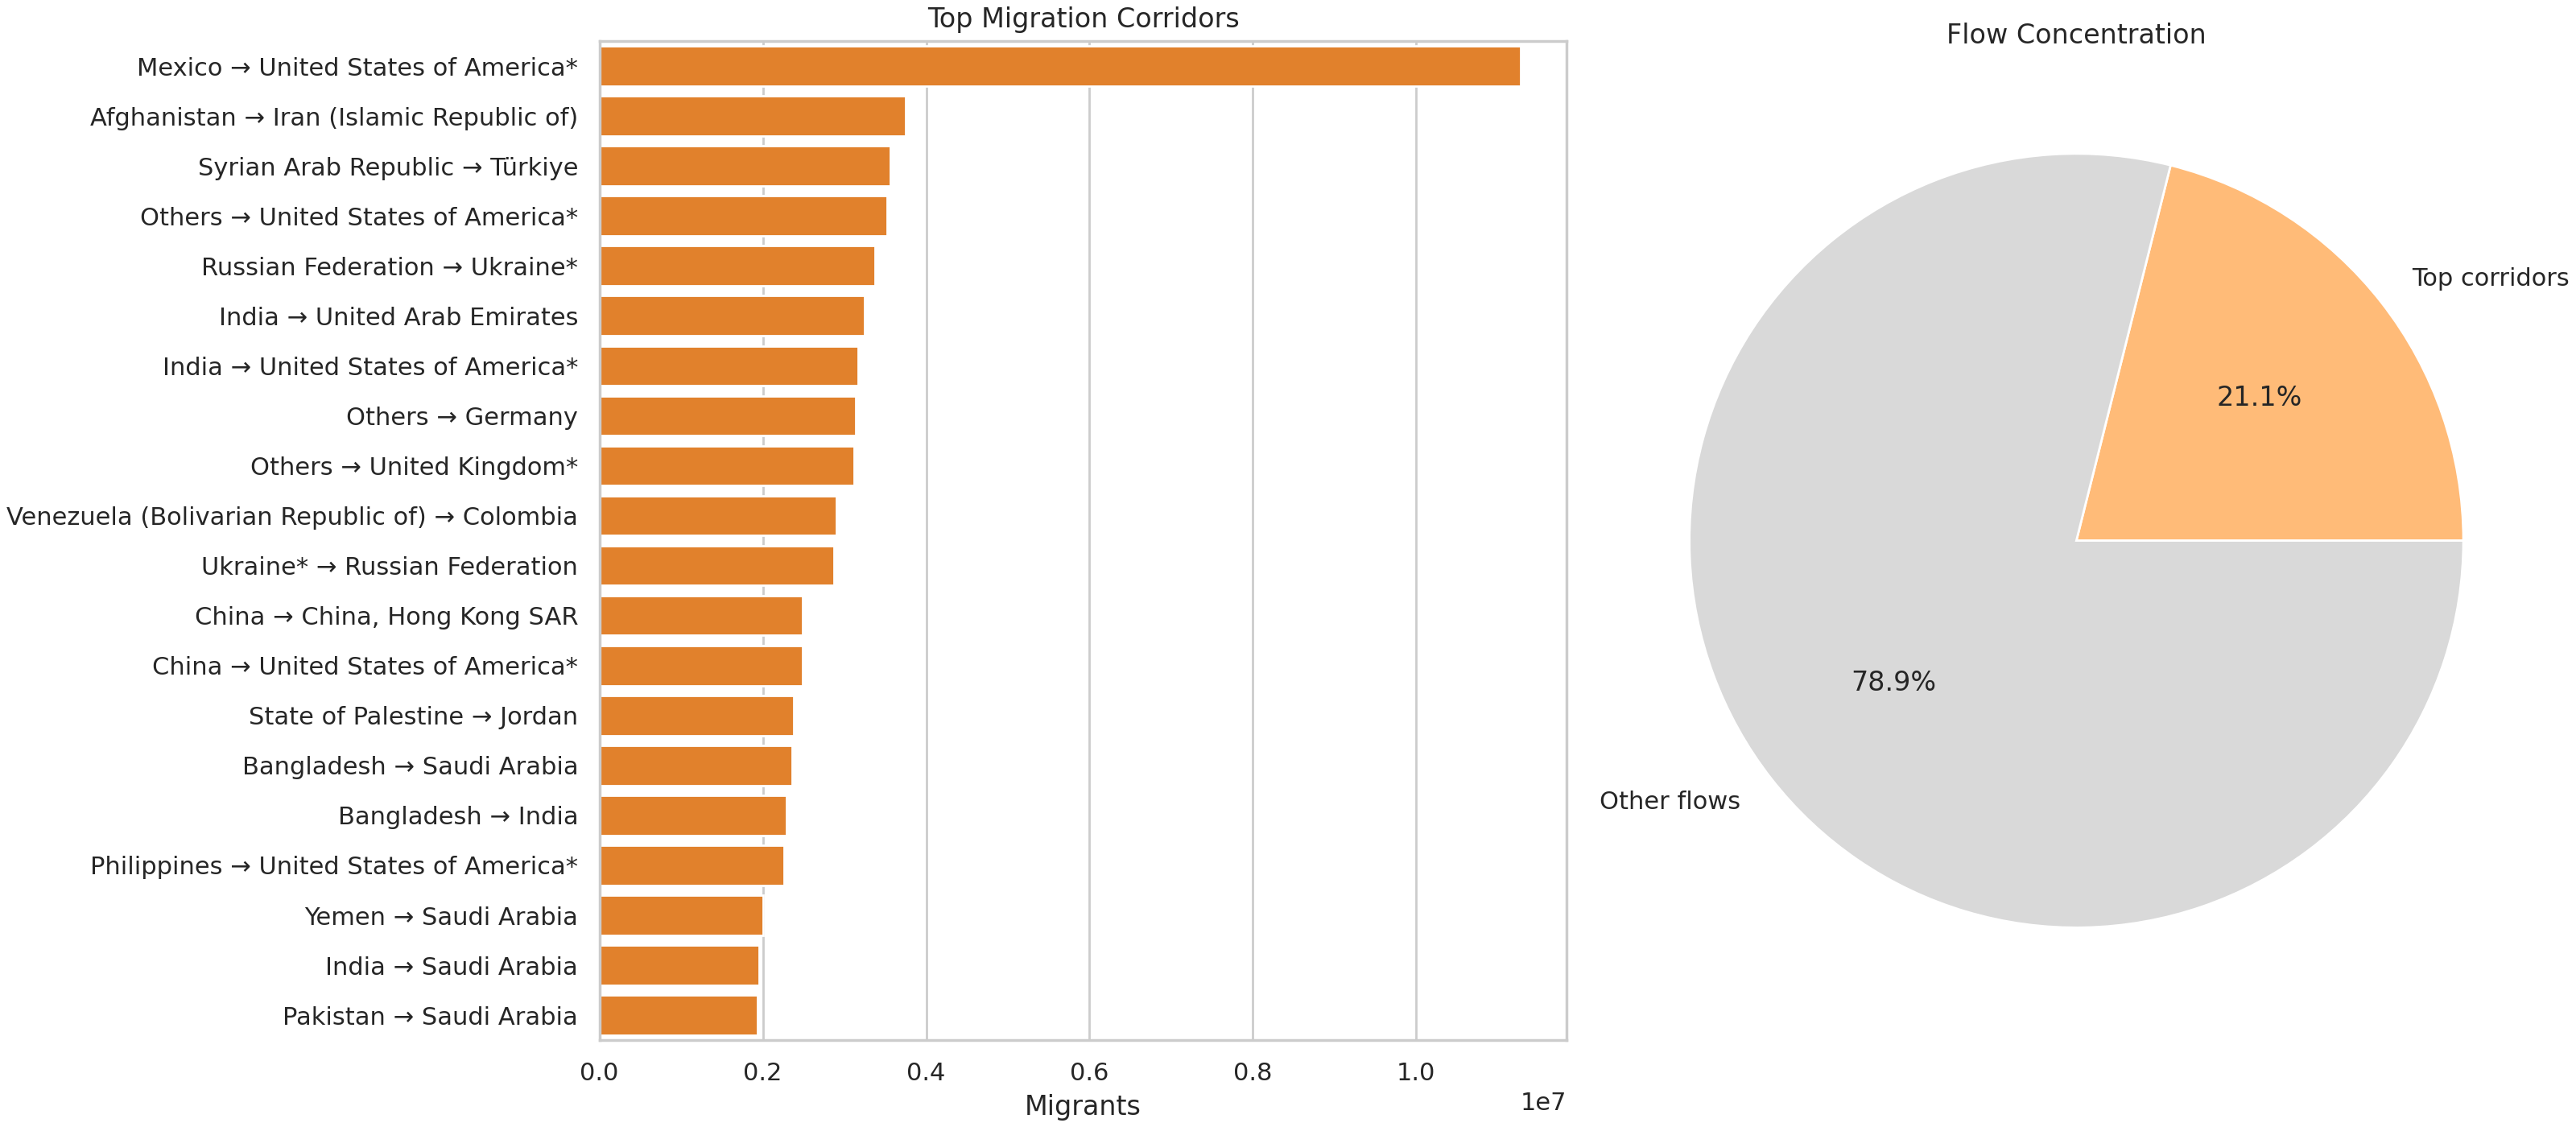
\includegraphics[width=0.9\textwidth]{deliverables_outputs/powerbi_exports/screenshots/dashboard_02_corridors.png}
  \caption{Top Migration Corridors Dashboard}
\end{figure}
\noindent\textit{Explanation:} Highlights the strongest bilateral flows and their distribution.

\begin{figure}[H]
  \centering
  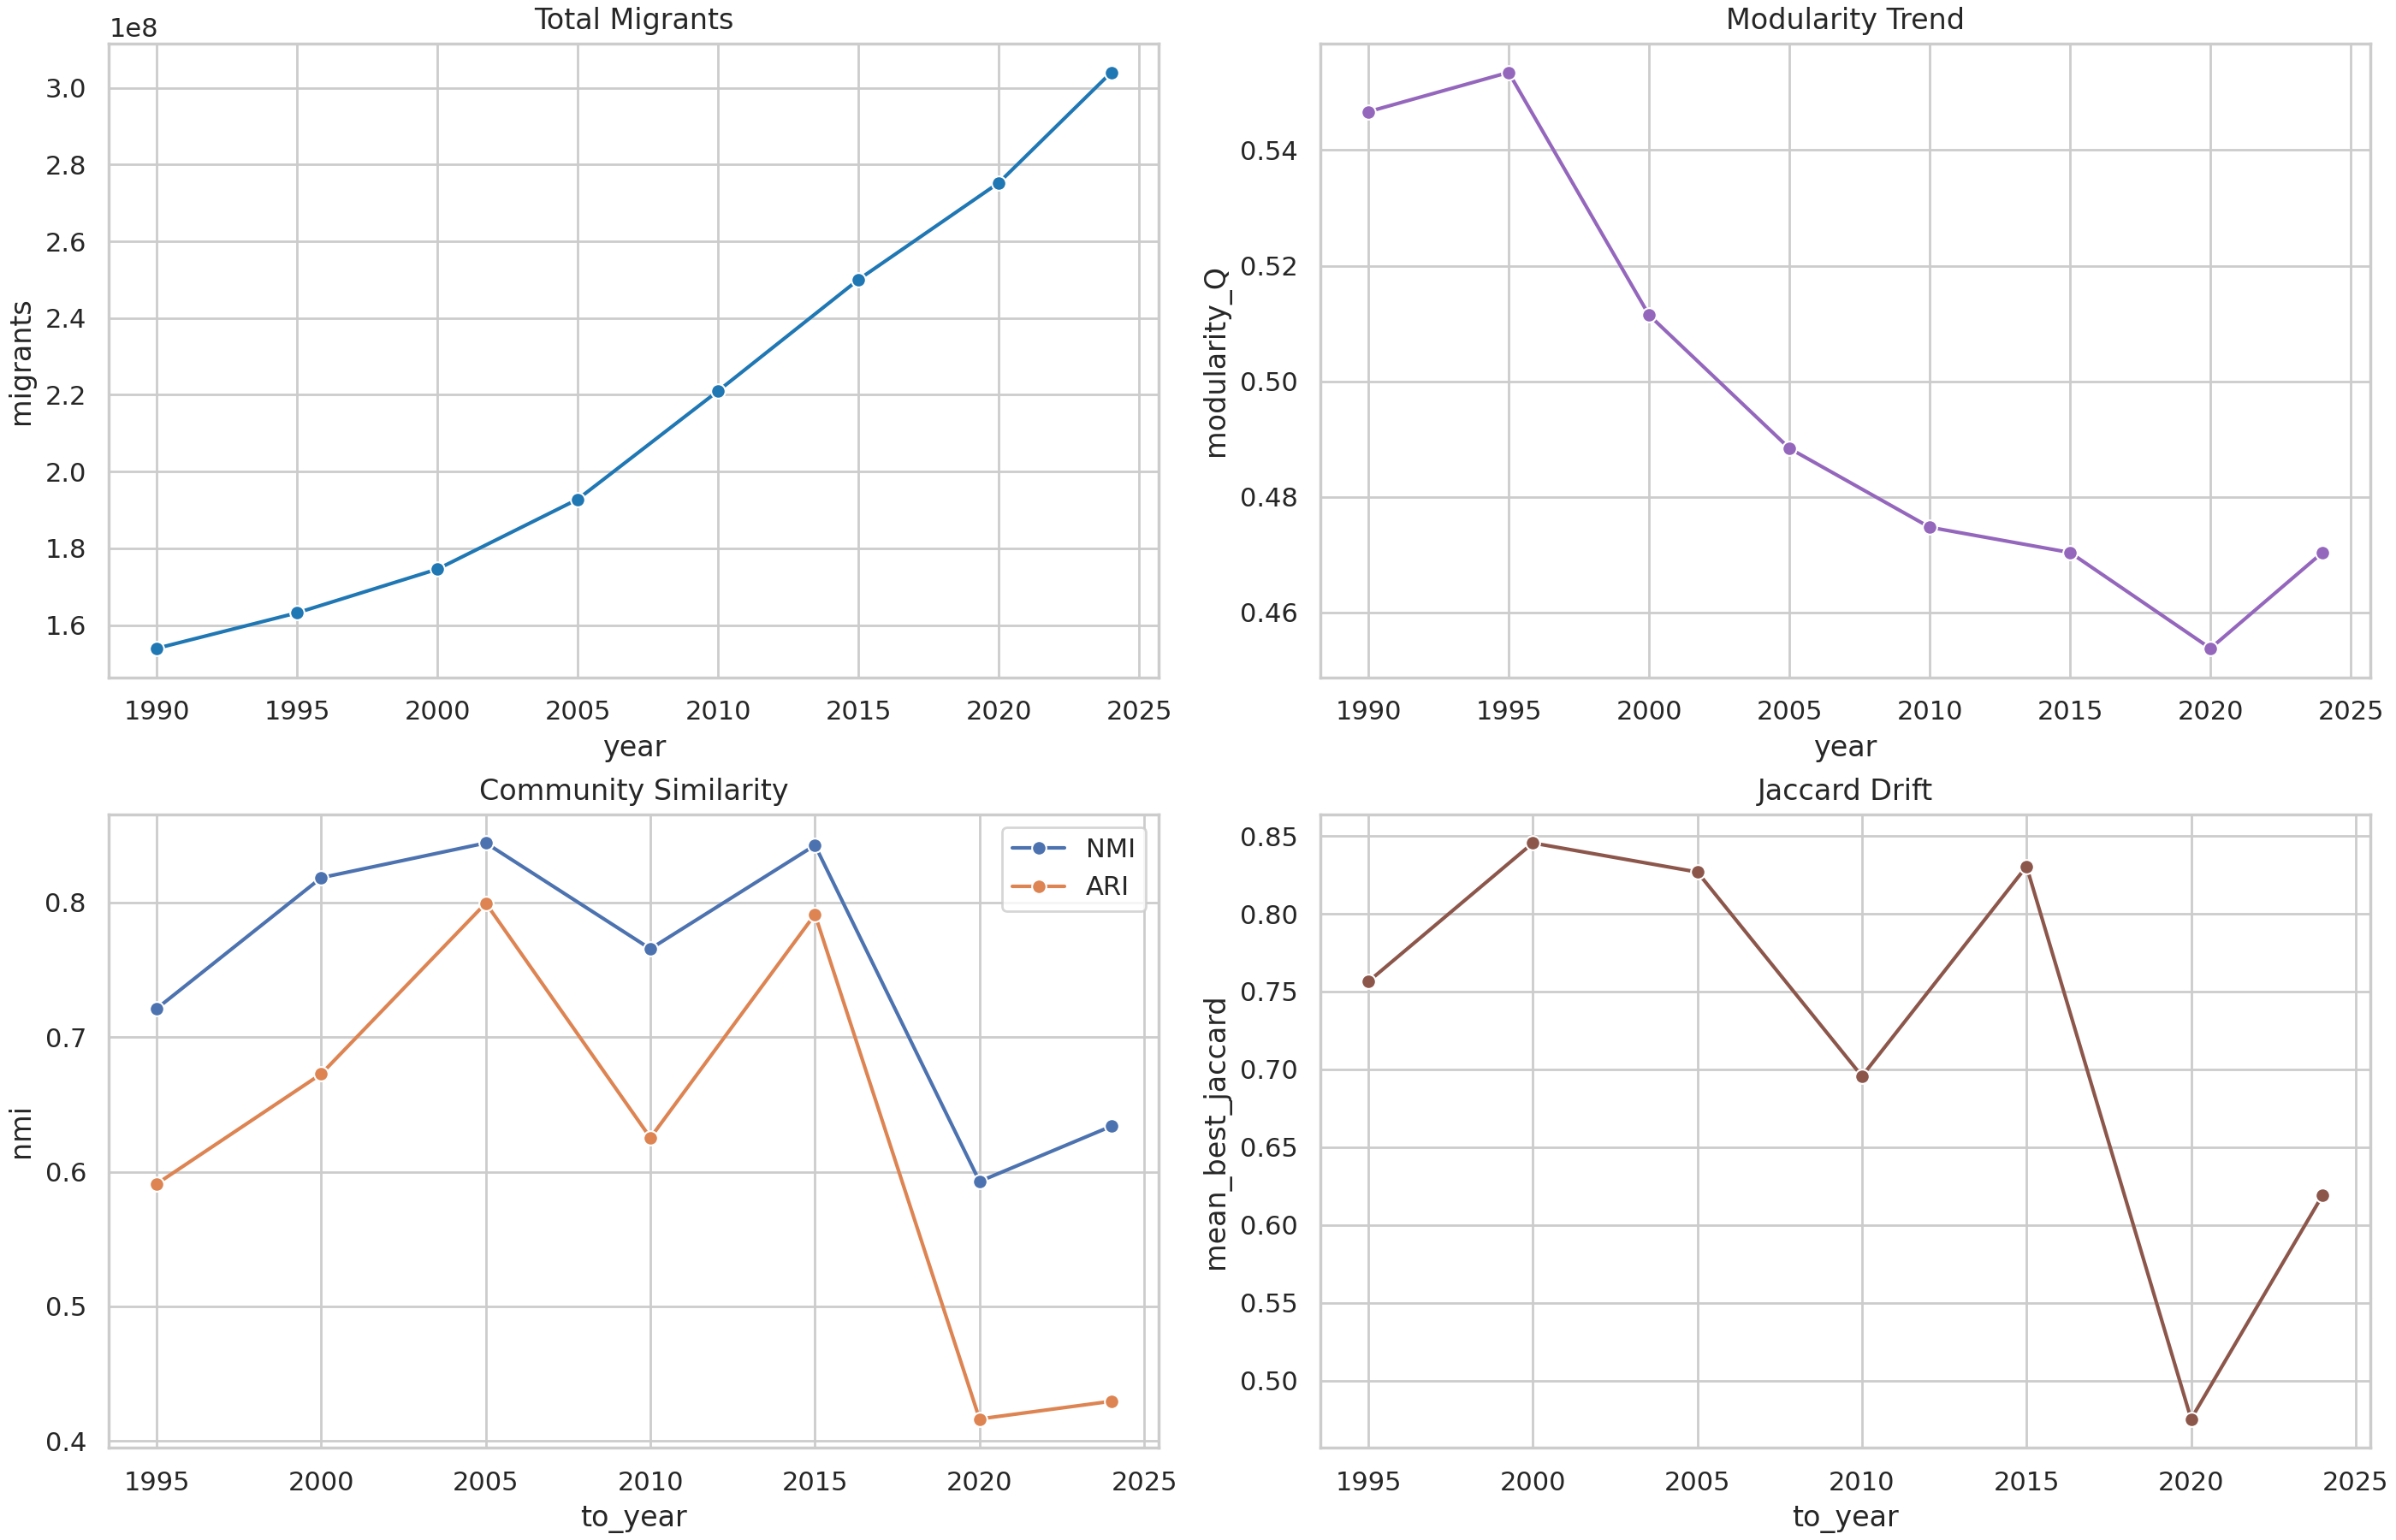
\includegraphics[width=0.9\textwidth]{deliverables_outputs/powerbi_exports/screenshots/dashboard_03_temporal.png}
  \caption{Temporal Trends Dashboard}
\end{figure}
\noindent\textit{Explanation:} Tracks total migrants over time alongside stability indicators.

\begin{figure}[H]
  \centering
  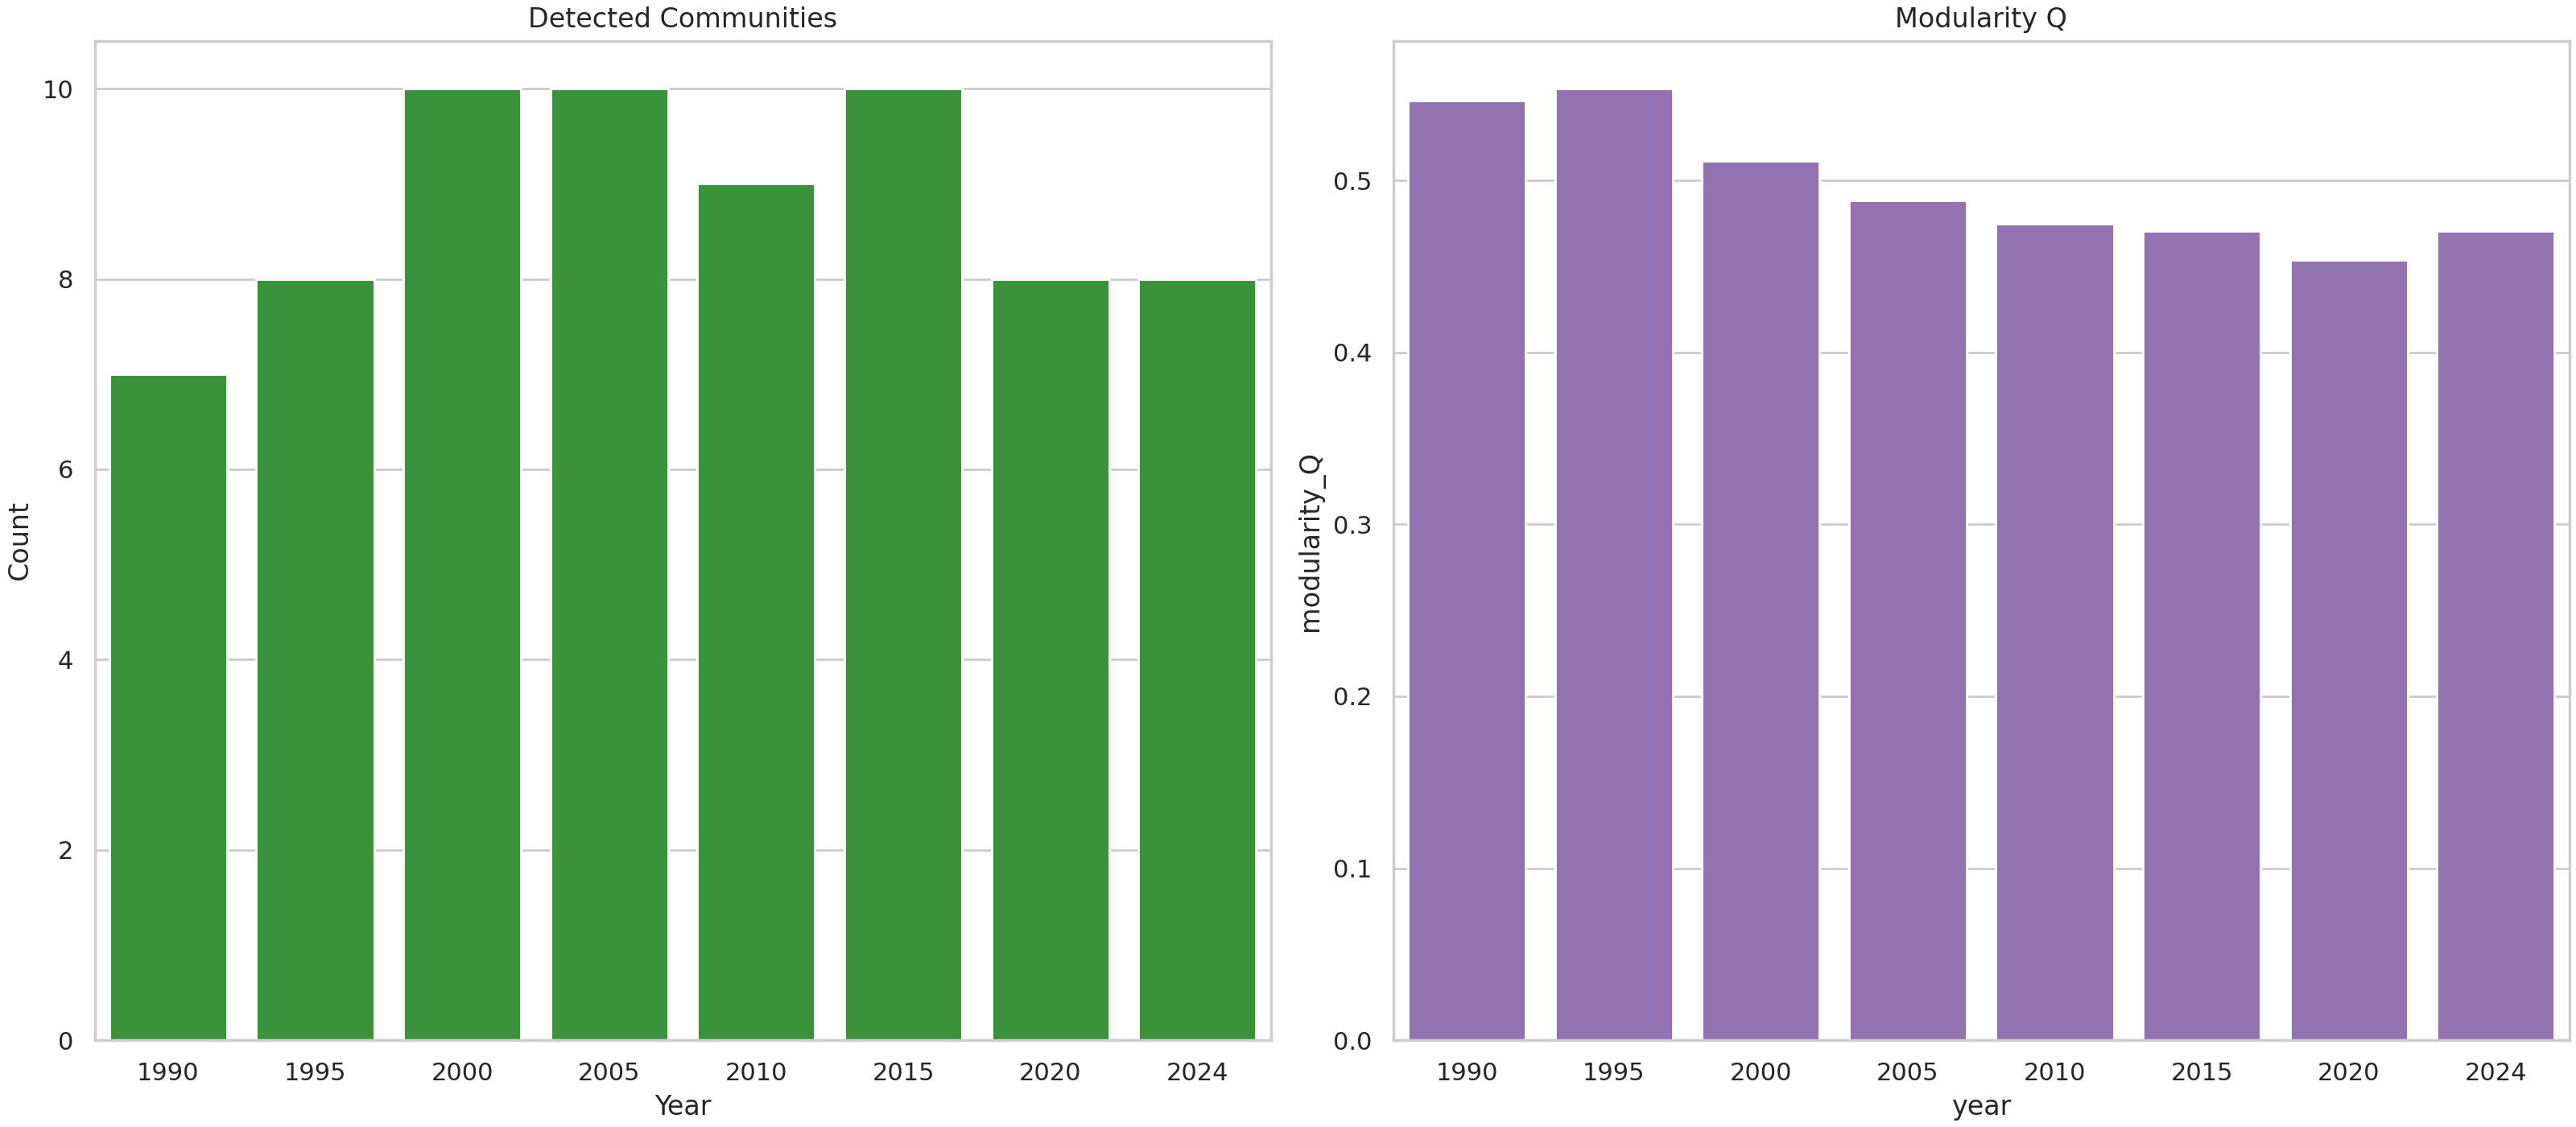
\includegraphics[width=0.9\textwidth]{deliverables_outputs/powerbi_exports/screenshots/dashboard_04_communities.png}
  \caption{Community Structure Dashboard}
\end{figure}
\noindent\textit{Explanation:} Displays the number of detected communities and modularity over time.

\begin{figure}[H]
  \centering
  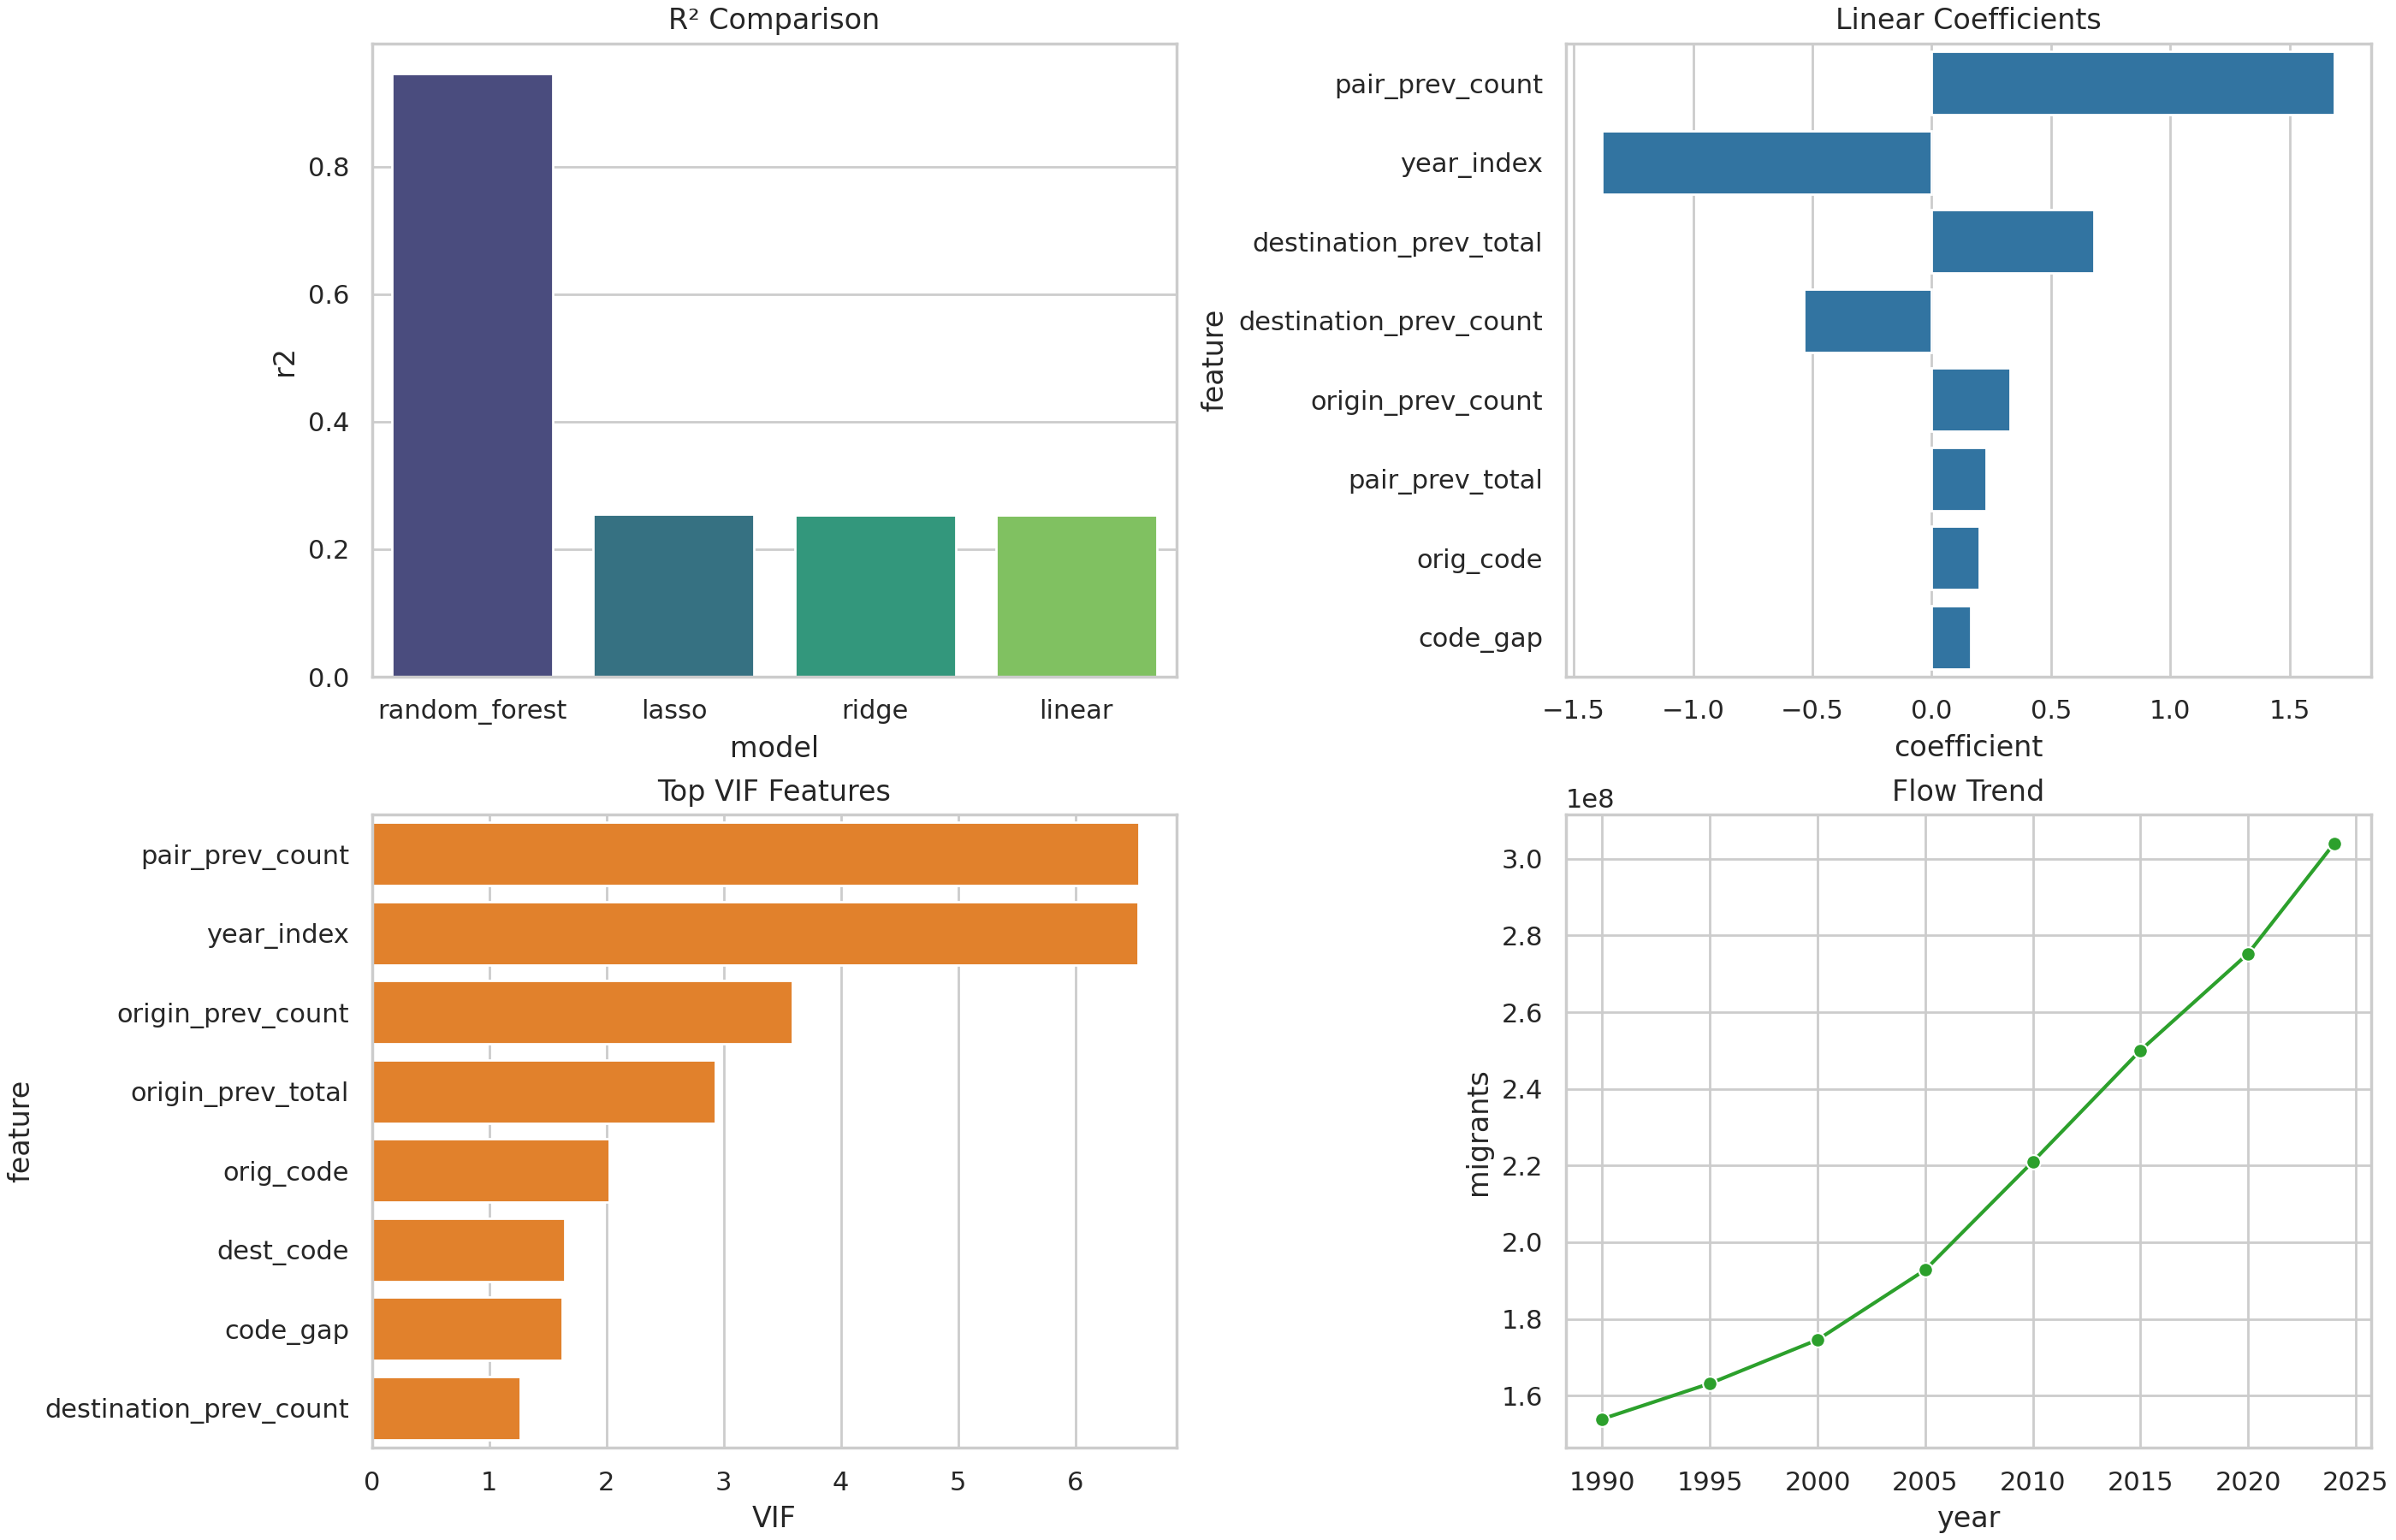
\includegraphics[width=0.9\textwidth]{deliverables_outputs/powerbi_exports/screenshots/dashboard_05_regression.png}
  \caption{Regression Diagnostics Dashboard}
\end{figure}
\noindent\textit{Explanation:} Shows model performance, coefficient patterns, and multicollinearity checks.

\chapter{Limitations and Future Work}
\section{Limitations}
\begin{itemize}
    \item Informal or undocumented migration is not fully captured.
    \item Auxiliary indicators are incomplete across countries and years.
    \item Community results are sensitive to algorithm choice.
    \item Policy shocks are not explicitly modeled.
\end{itemize}

\section{Future Work}
\begin{itemize}
    \item Integrate real-time migration APIs and administrative data.
    \item Apply Graph Neural Networks (GNNs) for prediction.
    \item Add climate and policy variables for scenario modeling.
    \item Extend forecasting to multi-scenario simulations.
\end{itemize}

\chapter{Conclusion}
This project demonstrates that combining network science with predictive modeling produces actionable migration insights. The centrality visualizations highlight persistent hubs, while the 5-year interval analysis reveals how migration intensifies across decades. Community stability metrics and the custom MIS score provide original insights into structural influence beyond raw volume. The final collage and dashboards deliver a clear, presentation-ready summary of findings for academic or policy audiences.

\chapter{References}
\begin{itemize}
    \item United Nations, Department of Economic and Social Affairs. \textit{International Migrant Stock 2024}.
    \item Newman, M. E. J. (2010). \textit{Networks: An Introduction}. Oxford University Press.
    \item Blondel, V. D., Guillaume, J.-L., Lambiotte, R., \& Lefebvre, E. (2008). Fast unfolding of communities in large networks.
    \item Traag, V. A., Waltman, L., \& van Eck, N. J. (2019). From Louvain to Leiden: guaranteeing well-connected communities.
\end{itemize}

\appendix
\chapter{Appendix A: Algorithm Summary}
\begin{longtable}{p{4cm}p{10cm}}
\toprule
Algorithm & Description \\
\midrule
Louvain & Modular community detection optimizing modularity. \\
Leiden & Improved modularity algorithm with well-connected communities. \\
Girvan--Newman & Edge-betweenness-based hierarchical community detection. \\
PageRank & Random-walk-based influence score. \\
Betweenness & Frequency of node on shortest paths. \\
\bottomrule
\end{longtable}

\chapter{Appendix B: Regression Features}
\begin{itemize}
    \item Pair historical totals and counts
    \item Origin and destination historical totals
    \item Year index and code gap
    \item Lag-based predictive features
\end{itemize}

\chapter{Appendix C: Output Artifacts}
\begin{itemize}
    \item Centrality tables per snapshot
    \item Community partitions and modularity tables
    \item Jaccard drift chart and NMI/ARI comparison tables
    \item Regression coefficient and VIF reports
    \item Dashboard-ready CSVs and screenshots
\end{itemize}

\end{document}
